\documentclass[11pt,a4paper]{article}
\usepackage{fontspec}
\setmainfont{TeX Gyre Pagella}
\newfontfamily\headfont{Inter}[UprightFont=*-ExtraBold,BoldFont=*-ExtraBold,Extension=.otf,Path=/usr/share/fonts/opentype/inter/]
\usepackage[a4paper,margin=2.3cm]{geometry}
\usepackage{graphicx,booktabs,float,caption,array,xcolor,longtable}
\usepackage{xurl}
\usepackage[hidelinks]{hyperref}
\usepackage{titlesec}
\usepackage[round]{natbib}
\usepackage{setspace}
\setstretch{1.05}
\renewcommand{\topfraction}{0.9}
\renewcommand{\bottomfraction}{0.8}
\renewcommand{\textfraction}{0.1}
\renewcommand{\floatpagefraction}{0.75}
\setlength{\parindent}{0pt}
\setlength{\parskip}{0.55em}
\titleformat{\section}{\headfont\Large}{\thesection}{0.8em}{}
\titleformat{\subsection}{\headfont\large}{\thesubsection}{0.8em}{}
\captionsetup{font=small,labelfont=bf}
\urlstyle{same}
\hypersetup{pdftitle={Al-Idrisi's World},pdfauthor={Tristan Hotham}}

\begin{document}
\begin{center}
{\Large\bfseries Al-Idrisi's World: The Map Made for Roger II of Sicily in 1154, Set Against a Modern Map\par}
\vspace{0.4em}
{\large 431 towns on Konrad Miller's reconstruction, measured for direction, distance, climate and scale, and compared with the Hereford Mappa Mundi\par}
\vspace{1.2em}
{\large Tristan Hotham\par}
\vspace{0.3em}
{\small Independent researcher\\
ORCID: 0000-0003-4931-9349\\
DOI: https://doi.org/10.5281/zenodo.23882607\par}
\vspace{0.8em}
2026
\end{center}

\begin{quote}
\small
\begin{center}\textbf{Abstract}\end{center}
Al-Idrisi's world map, finished in Palermo in 1154 for Roger II of Sicily, is drawn with south at the top on a grid of seven climates and ten sections. I located 431 legible town labels on Konrad Miller's 1928 reconstruction of the map, identified each with a modern place, checked the positions against three gazetteers, and measured how the map, turned north up, distorts the world. Directions are well kept: across 92,193 pairs of towns at least 100 km apart the median error in bearing is 10 degrees and 99\% lie within 45 degrees. The best affine fit of the whole map puts the median town 239 km from its real position. Locally the map is more faithful: the median distance between a town and the position predicted from its eight nearest neighbours is 55 km, rising from 44 km around the Mediterranean to 71 km in northern Europe and 92 km in Asia beyond the Euphrates. Sicily is both the most faithfully drawn region (21 km) and the most enlarged (1.42 times the map's average scale). The climates keep the order of latitude but not its spacing: the boundaries implied by the towns fall at about 18.0, 28.6, 35.8, 40.4, 47.3 and 53.2 degrees north. 63 route distances from Dozy and de Goeje's 1866 edition give a median of 1.42 km of straight line per stated mile and about 36 km per day stage. Measured exactly as in my study of the Hereford Mappa Mundi (about 1300), al-Idrisi's map explains 0.94 of the spread of real positions about Jerusalem against 0.84, with a median miss of 330 km against 516 km.

\textbf{Keywords:} medieval cartography; Islamic geography; al-Idrisi; Tabula Rogeriana; Roger II; map distortion; climates; historical gazetteers; open data
\end{quote}

\section{Introduction}
Abu Abd Allah Muhammad al-Idrisi, born in Ceuta, worked at the court of Roger II, the Norman king of Sicily, and in 1154 completed for him a geography, the \textit{Nuzhat al-mushtaq}, often called the Book of Roger, together with a world map. The work divides the inhabited world into the seven climates of Greek and Islamic geography, bands of latitude from the equator northward, and each climate into ten sections from west to east; each of the seventy sections has its own description and its own sheet. Joined, the sheets form a rectangular map of the world with south at the top. The original is lost; the map is known from manuscript copies of the section maps, which Konrad Miller assembled into a single reconstruction in 1928 \citep{miller1928}.

This paper sets that reconstruction against a modern map. It asks how well the map keeps direction and distance; where it is most and least faithful; whether its climates follow latitude; how it treats the Nile and Britain; how its book's stated distances compare with real ones; and how it compares, on the same measures, with the Hereford Mappa Mundi, a Christian world map drawn about 146 years later, which I analysed in an earlier study \citep{hereford}. It accompanies an interactive comparison (\url{https://maps.tristanhotham.com/idrisi/}).

\section{Data}
\textbf{The map.} Miller's reconstruction \citep{miller1928}, from Wikimedia Commons (public domain), scanned at 12,999 by 5,958 pixels. Miller redrew the map from the manuscripts and transcribed every name into Latin letters; all positions in this study are therefore positions on Miller's sheet, not on a medieval manuscript.

\textbf{The text.} \citet{dozy} edited and translated the parts of the Book of Roger on North Africa and Spain. The Internet Archive's text of that edition (public domain) supplies the route distances.

\textbf{Gazetteers.} al-Thurayya \citep{thurayya}, a gazetteer of the places and routes of the early Islamic world with modern coordinates, derived from Cornu's atlas (CC BY 4.0); Pleiades \citep{pleiades}, version 4.1 (CC BY 3.0); and Natural Earth countries and populated places \citep{naturalearth}.

\section{Methods}
\subsection{Reading and locating towns}
Miller drew settlements as small brown discs with spokes, each beside its transcribed name. I read the labels section by section at full resolution and recorded, for each town I could read and identify with confidence, the pixel of its disc and my confidence (362 read clearly, 69 with some doubt because the label is crowded, faded or ambiguous). I left out rivers, mountains, regions and peoples, and every label I could not identify. To make positions reproducible I detected the discs automatically, first by shape (a colour mask, a morphological opening and a test for round blobs of the right size) and then by matching a template built from the clean discs; 5,329 candidate discs were found, and 386 of my readings (90\%) were snapped to a disc within 20 pixels, a median 1.9 pixels away. Readings left unsnapped were checked by eye on close-up images, and eleven positions were corrected in this way.

\subsection{Modern positions}
I gave each identification a modern position and checked it against the three gazetteers by name: al-Thurayya by Miller's transliteration and by the identification, Pleiades by attested and romanised names, Natural Earth by modern names. 365 of the 431 towns (85\%) matched a gazetteer entry of the same name within 150 km, at a median distance of 0.7 km from my position (178 in al-Thurayya, 264 in Pleiades, 196 in Natural Earth); every match more than 30 km away was reviewed. The towns not matched are small places the gazetteers do not list. Each town was assigned to one of 18 regions (Table~\ref{tab:regions}).

\subsection{Measures}
All measures use the map turned through 180 degrees, so that north is up. The \textit{global fit} is the affine map (least squares) from map position to longitude and latitude; the \textit{residual} of a town is the great circle distance between its real position and its fitted position. The \textit{local error} of a town is obtained by fitting an affine map from map position to an azimuthal equidistant projection centred on the town, using only its eight nearest neighbours by true distance, and measuring how far that fit puts the town from its real position; it measures how well the map keeps the shape of each neighbourhood, regardless of distortion at the scale of the whole map. For each region with at least five towns I also computed, over all pairs of towns in the region at least 100 km apart, the median absolute difference between the bearing on the map and the true initial bearing, and the median ratio of map distance to true distance relative to the same median over all pairs on the map (the \textit{stretch}, as in the Hereford study). Because the map is a rectangular grid, stretch was also computed for a perfect rectangular grid with the fitted ratio of degrees of longitude to degrees of latitude, to separate the effect of the grid from the mapmaker's choices.

The climate of each town is read from Miller's red climate lines, located automatically in each of the ten sections. For each pair of neighbouring climates, the \textit{implied boundary} is the latitude that best separates the towns of the two climates. For the comparison with Hereford I repeated that study's method exactly: the similarity transform (rotation, uniform scale and shift) that best lays the map positions on an azimuthal equidistant projection centred on Jerusalem, and bearings from Jerusalem on the map and on the globe.

\subsection{Route distances}
From \citet{dozy} I took 63 distances stated between two places I could identify, over land or along a coast: 37 in miles and 30 in day stages (some give both). Each was checked against the line of the scan's text it comes from, which is recorded in the data. I compared each with the great circle distance between the places.

\section{Results}
\subsection{The towns and the whole-map fit}
Figure~\ref{fig:maps} shows the 431 towns on the map and on a modern map. The global affine fit explains 0.98 of the variance in longitude and 0.90 in latitude. It draws a degree of longitude 0.93 times as long as a degree of latitude, the ratio of a rectangular grid true to scale at about 21 degrees north. The median residual is 239 km, 54\% of towns are within 250 km of their fitted position and 88\% within 500 km (Figure~\ref{fig:arrows}).

\begin{figure}[tbp]\centering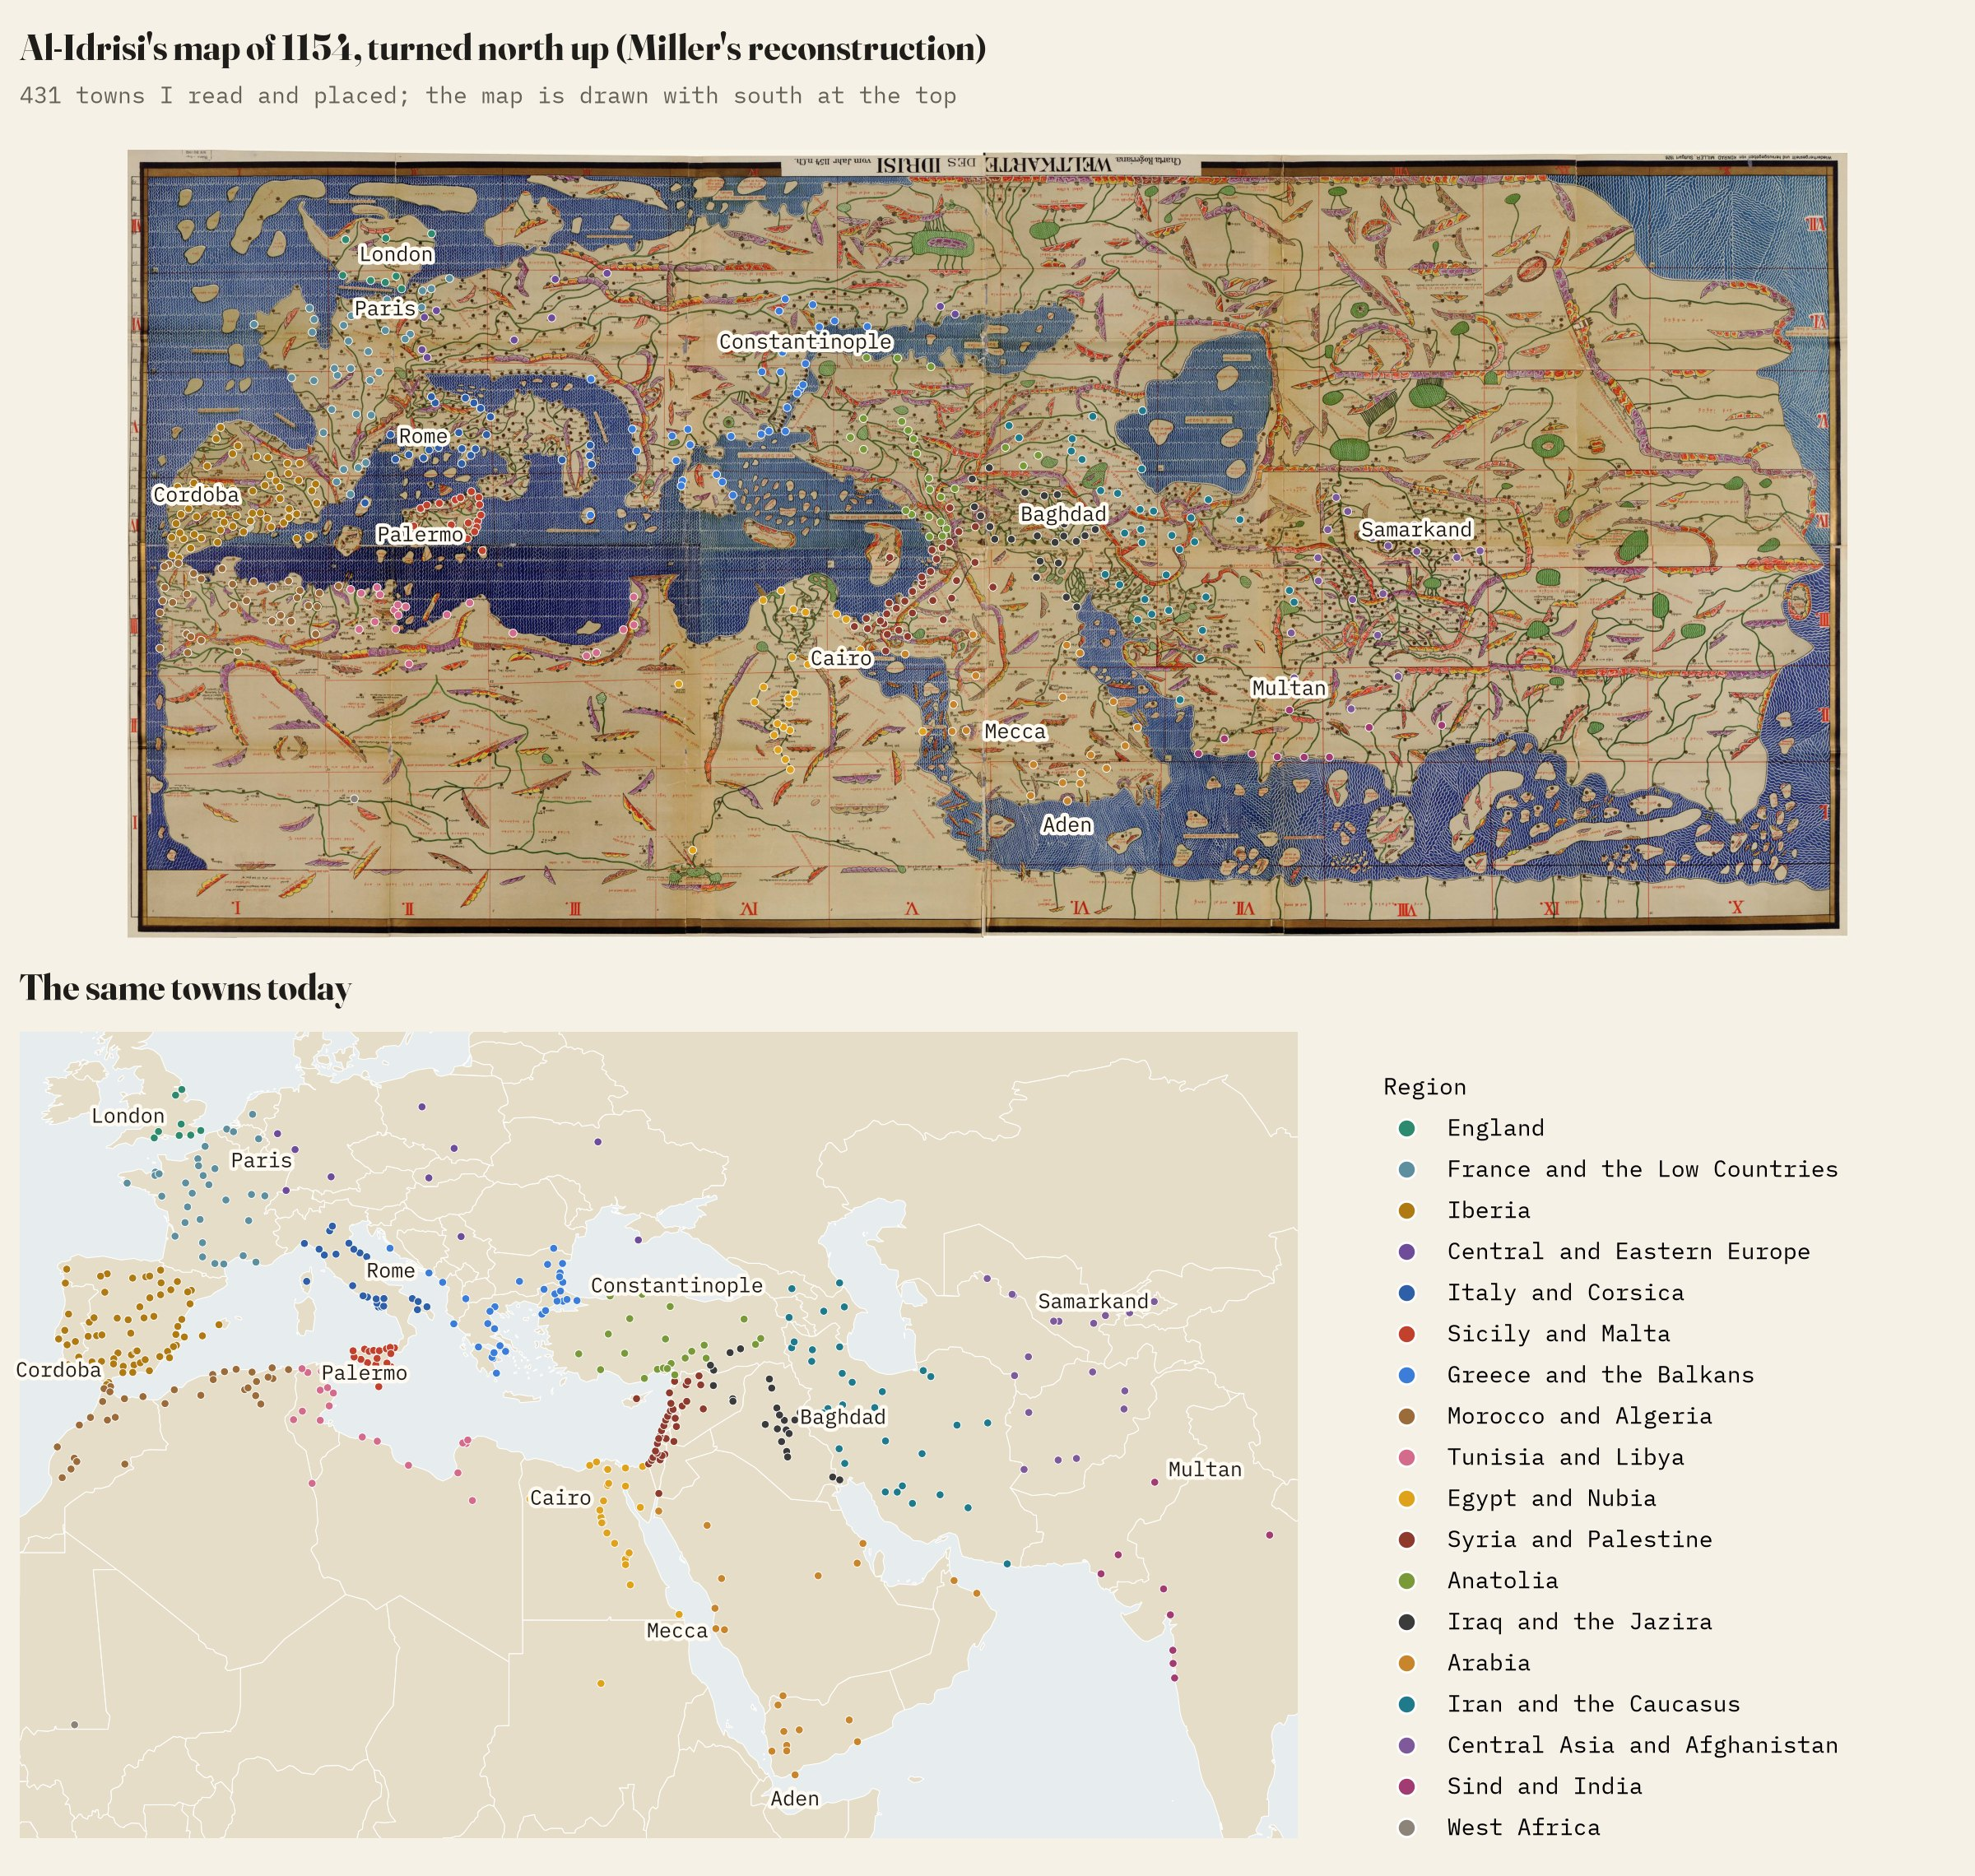
\includegraphics[width=\textwidth]{f_maps.jpg}
\caption{The located towns on Miller's reconstruction, turned north up (top), and on a modern map (bottom), coloured by region.}\label{fig:maps}\end{figure}

\begin{figure}[tbp]\centering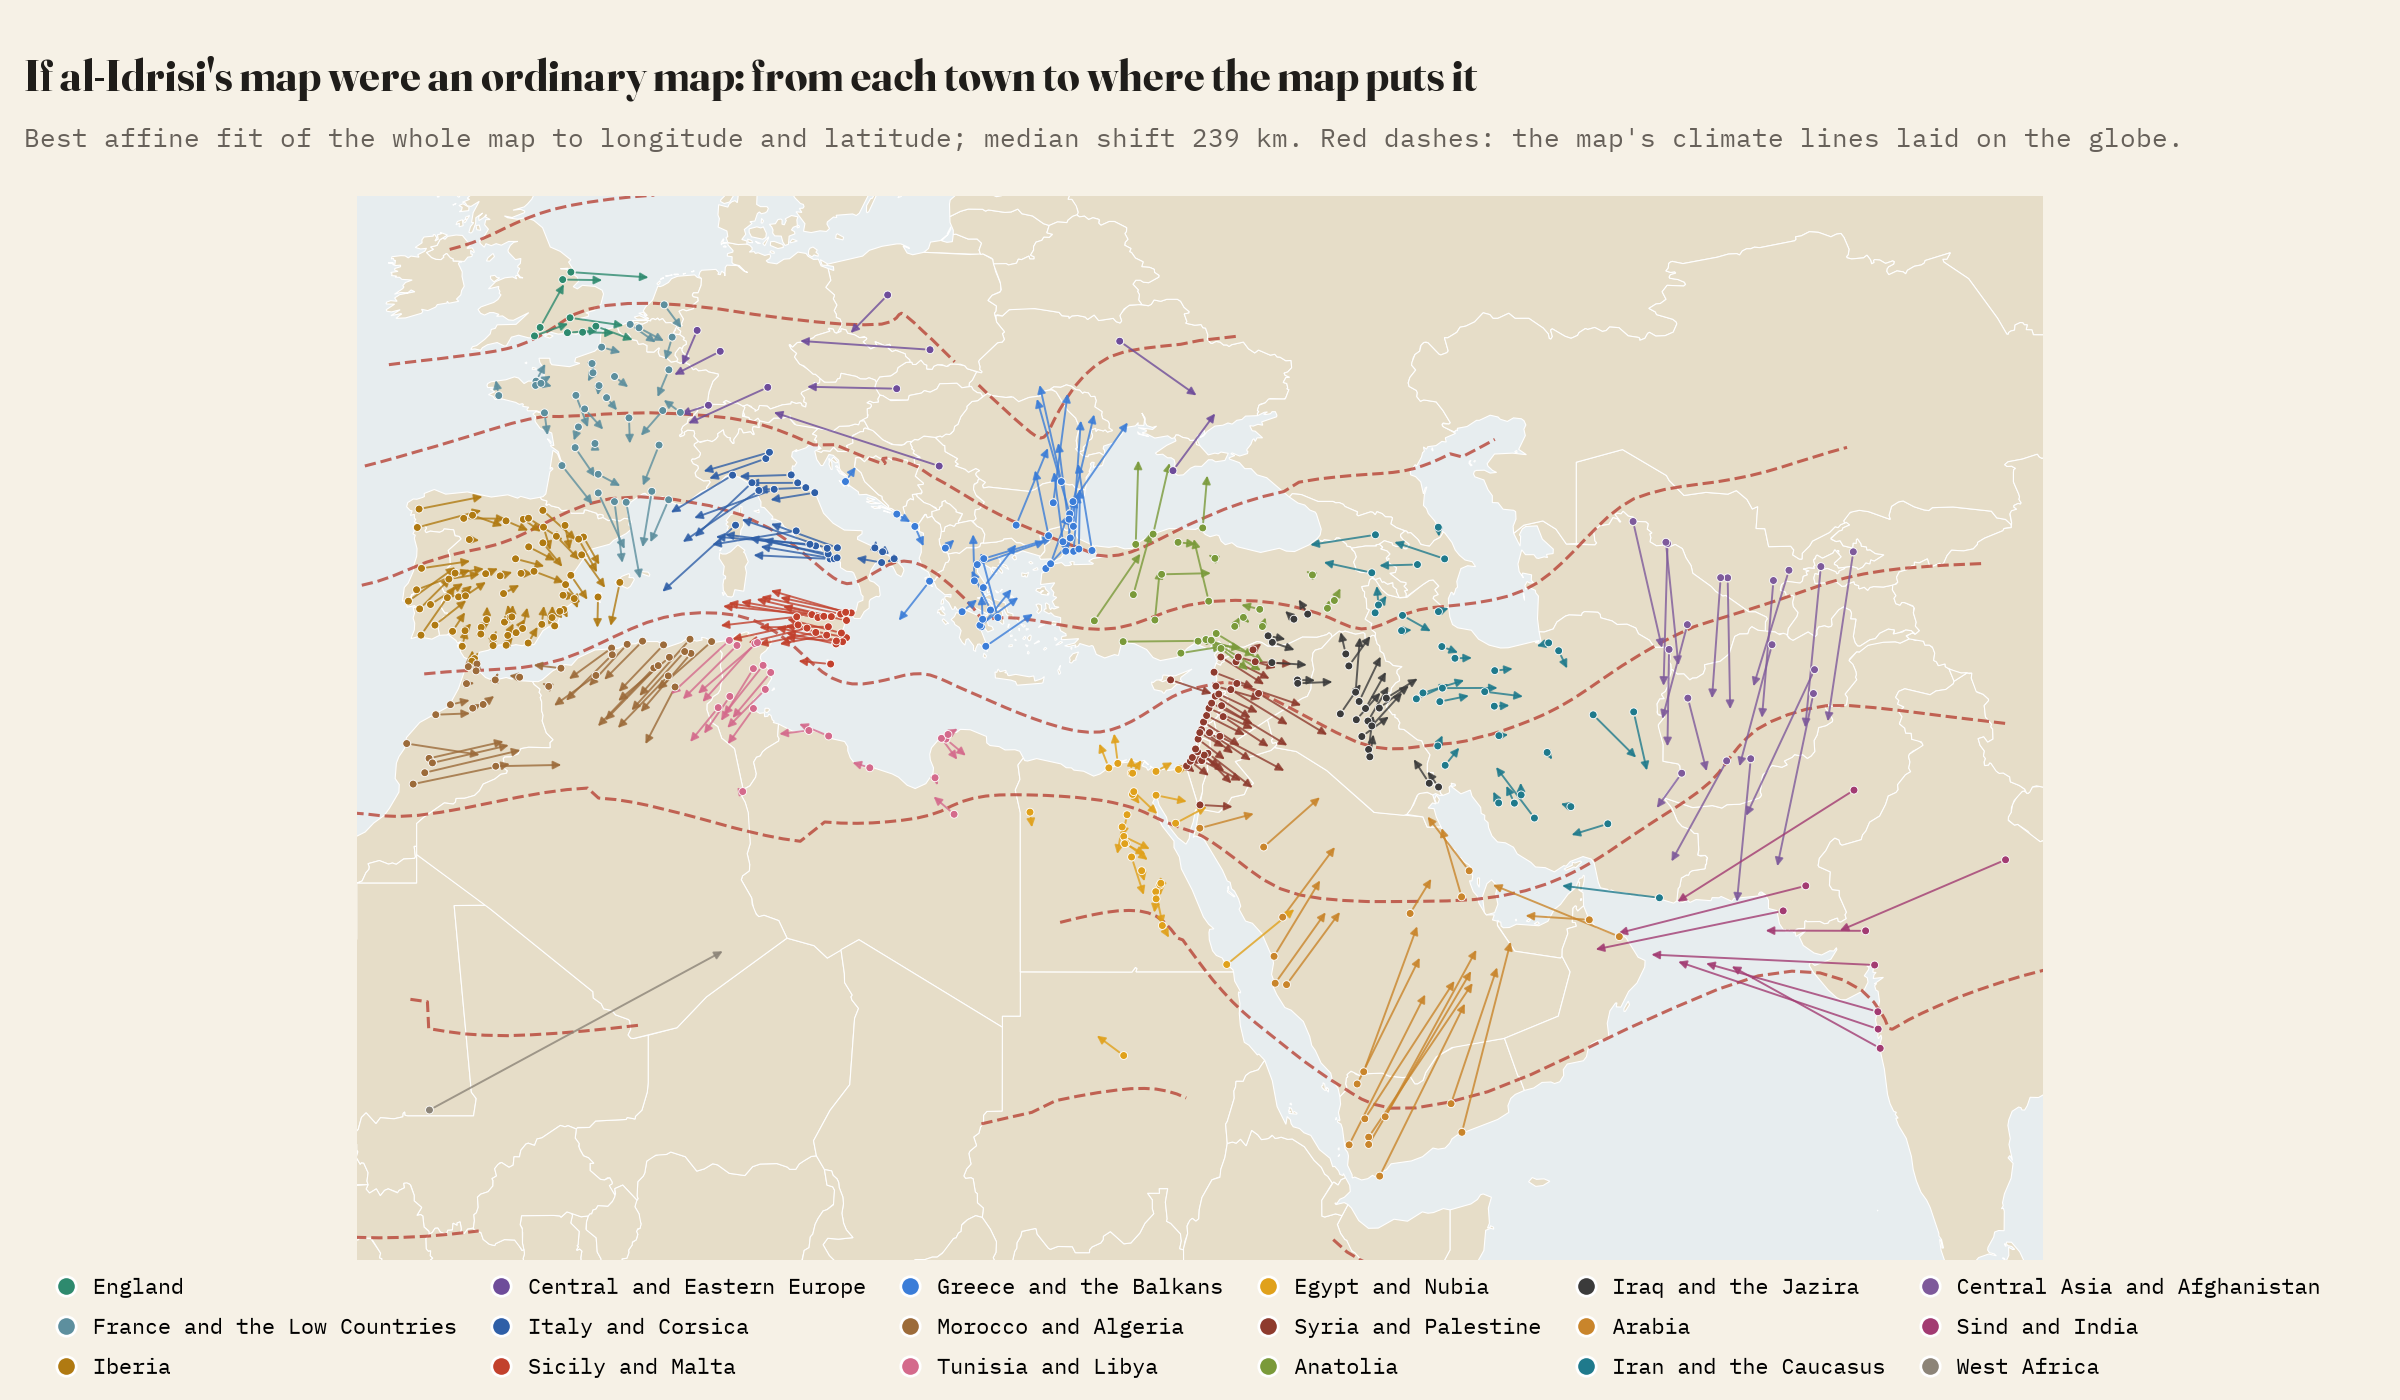
\includegraphics[width=\textwidth]{f_arrows.png}
\caption{From each town to its position under the best affine fit of the whole map, with the map's climate lines carried onto the globe.}\label{fig:arrows}\end{figure}

\subsection{Direction and local shape}
Directions are well kept. Across all 92,193 pairs of towns at least 100 km apart, the median bearing error is 10 degrees and 99\% are within 45 degrees; the rank correlation between map and true distance is 0.95. The median local error is 55 km, with 76\% of towns within 100 km and 91\% within 200 km. Table~\ref{tab:regions} and Figure~\ref{fig:regions} give the figures by region. The most faithful regions are Sicily (21 km), Syria and Palestine (26 km), Morocco and Algeria and Iberia (37 km each), and Italy (38 km); the least faithful are Arabia (156 km), central and eastern Europe (212 km) and Sind and India (247 km). Grouped, the Mediterranean regions have a median local error of 44 km (275 towns), northern Europe 71 km (50) and Asia beyond the Euphrates 92 km (105).

\begin{table}[tbp]\centering\small\caption{Located towns by region: number, median local error (km), median residual of the global affine fit (km), median bearing error between pairs (degrees), stretch relative to the map's average scale, and the stretch a perfect rectangular grid would give. Blank: fewer than five towns.}\label{tab:regions}\begin{tabular}{lrrrrrr}\toprule Region & Towns & Local & Global & Bearing & Stretch & Grid\\\midrule
England & 8 & 63 & 175 & 39 & 1.25 & 0.98\\
France and the Low Countries & 32 & 57 & 143 & 18 & 1.18 & 1.00\\
Iberia & 64 & 37 & 140 & 23 & 0.84 & 0.99\\
Central and Eastern Europe & 10 & 212 & 379 & 15 & 0.92 & 1.16\\
Italy and Corsica & 24 & 38 & 369 & 25 & 1.25 & 1.01\\
Sicily and Malta & 20 & 21 & 362 & 28 & 1.42 & 0.99\\
Greece and the Balkans & 32 & 76 & 315 & 20 & 1.38 & 0.99\\
Morocco and Algeria & 33 & 37 & 353 & 19 & 0.68 & 0.99\\
Tunisia and Libya & 20 & 50 & 253 & 18 & 0.93 & 0.95\\
Egypt and Nubia & 25 & 61 & 156 & 17 & 1.13 & 0.89\\
Syria and Palestine & 33 & 26 & 249 & 20 & 1.25 & 0.90\\
Anatolia & 24 & 87 & 253 & 20 & 1.04 & 1.00\\
Iraq and the Jazira & 23 & 54 & 204 & 22 & 0.87 & 0.93\\
Arabia & 21 & 156 & 759 & 17 & 0.59 & 0.88\\
Iran and the Caucasus & 34 & 81 & 128 & 17 & 0.86 & 0.92\\
Central Asia and Afghanistan & 18 & 137 & 669 & 24 & 0.84 & 0.94\\
Sind and India & 9 & 247 & 1,112 & 39 & 0.73 & 0.88\\
West Africa & 1 & 664 & 1,921 &  &  & \\
\bottomrule\end{tabular}\end{table}

\begin{figure}[tbp]\centering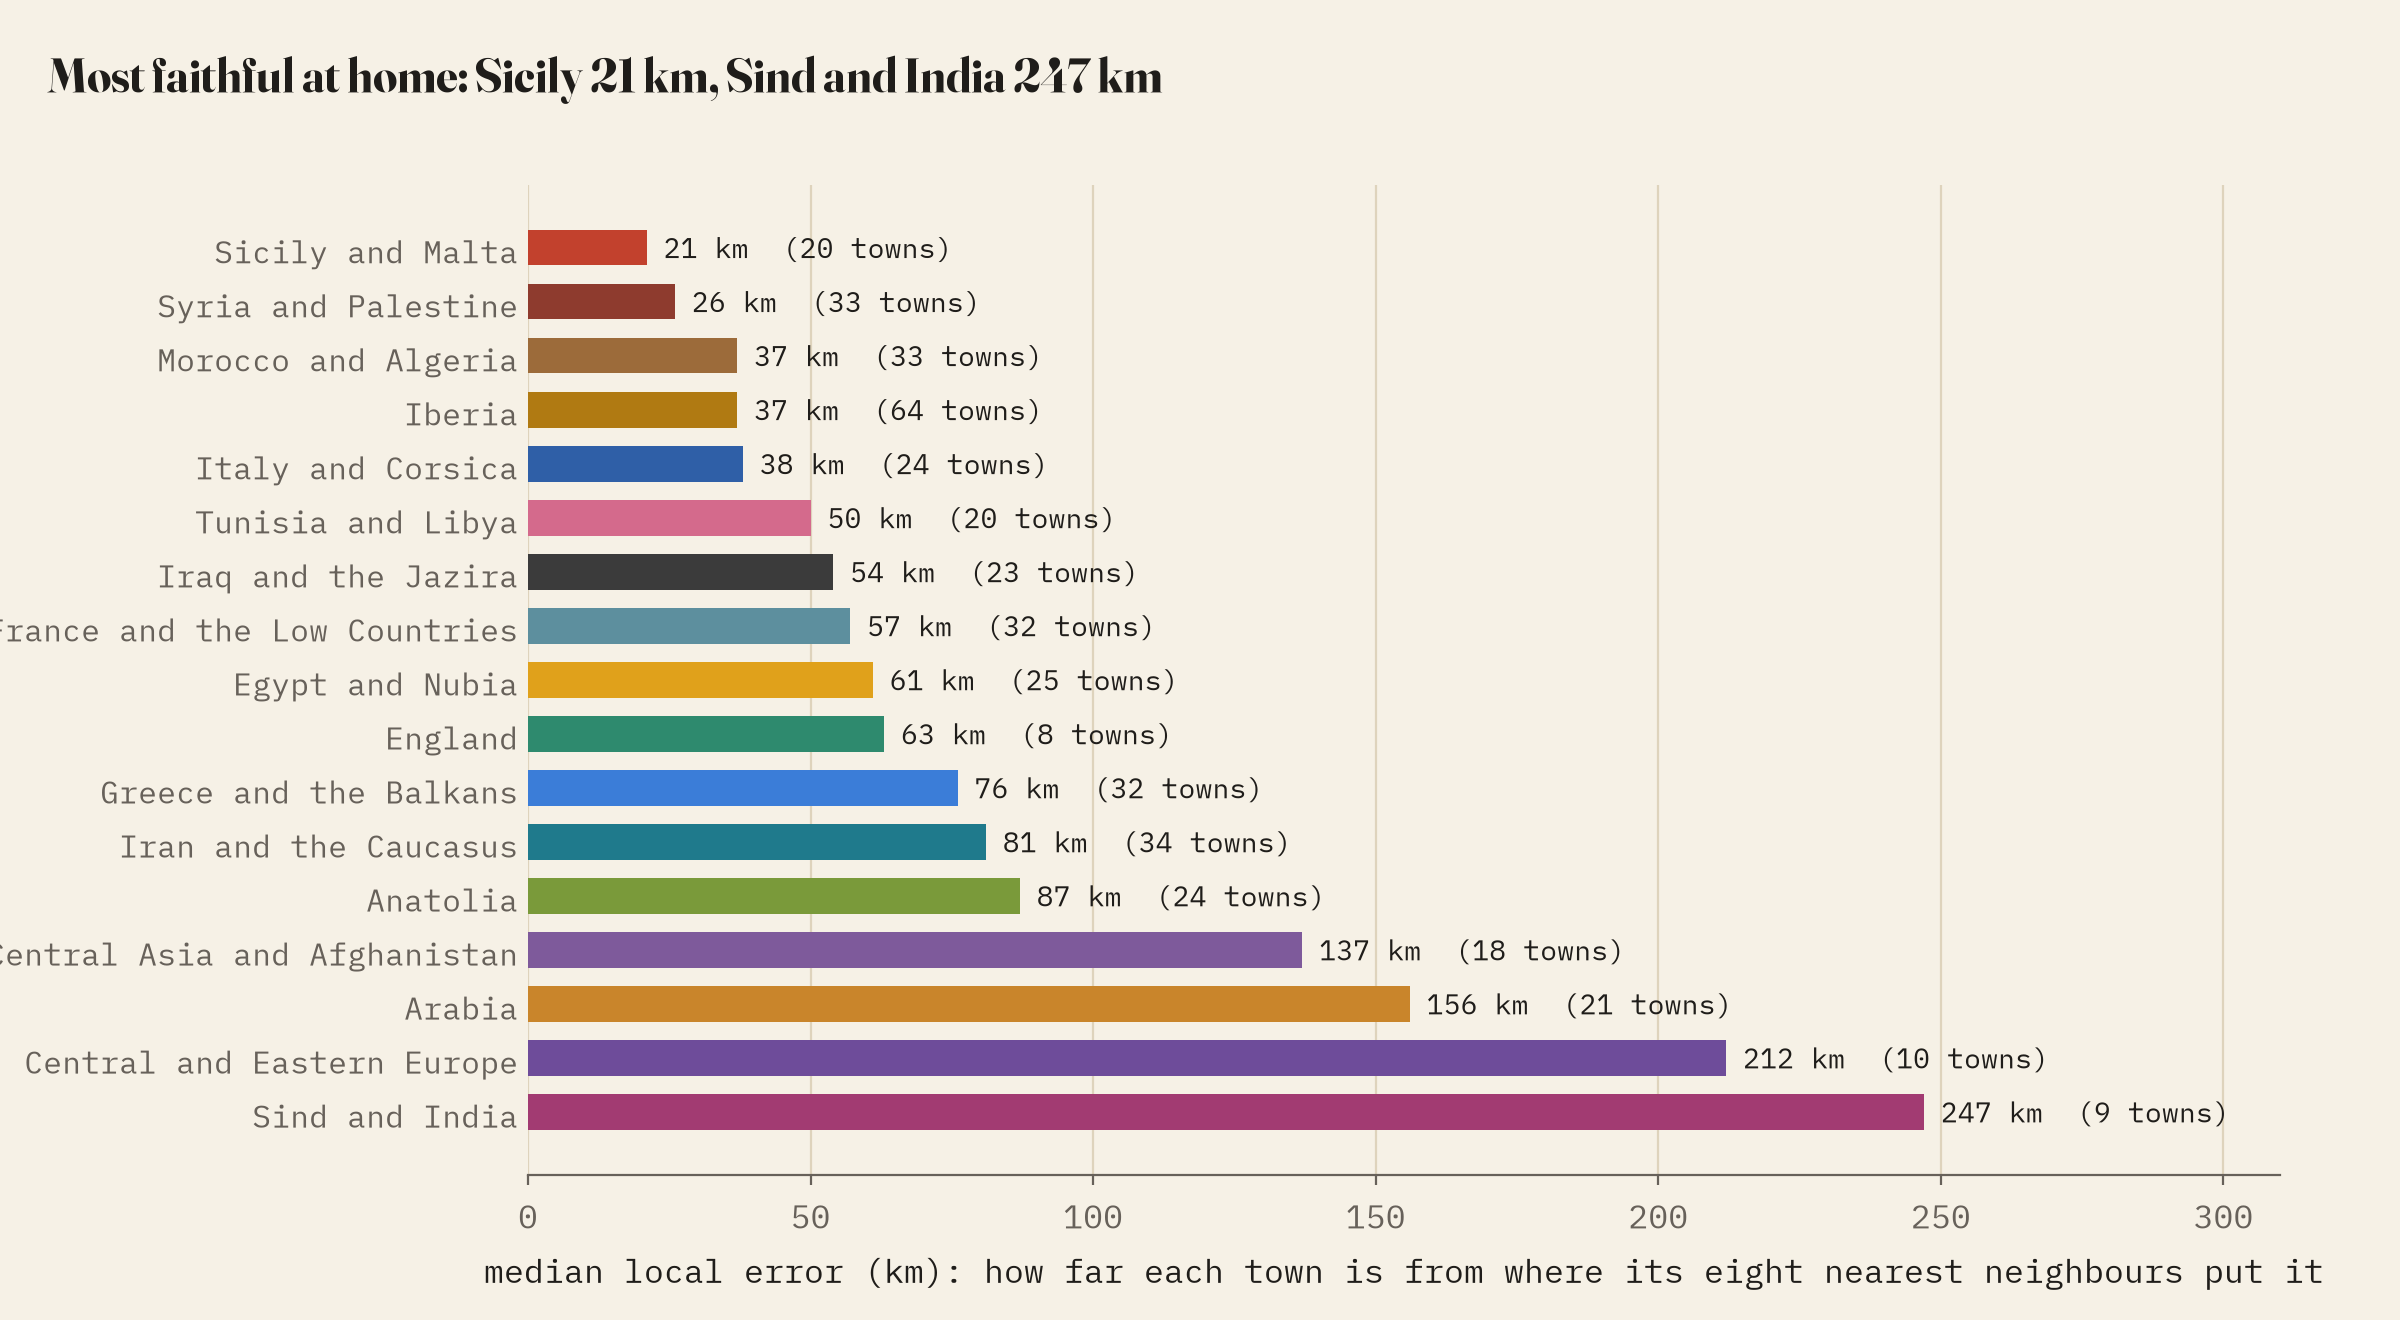
\includegraphics[width=\textwidth]{f_regions.png}
\caption{Median local error by region: the distance from each town to the position predicted by an affine fit to its eight nearest neighbours.}\label{fig:regions}\end{figure}

\subsection{Scale and Sicily}
Relative to the map's average scale, Sicily is drawn largest (1.42), followed by Greece and the Balkans (1.38), England and Italy (1.25) and Syria and Palestine (1.25); Morocco and Algeria (0.68) and Arabia (0.59) are drawn smallest. A perfect rectangular grid with the map's proportions would leave Sicily at 0.99, so its enlargement is not an artefact of the grid. The local fit for Sicily is rotated by about 31 degrees, which explains why its bearing error (28 degrees) is among the highest even though its local error is the lowest (Figure~\ref{fig:sicily}).

\begin{figure}[tbp]\centering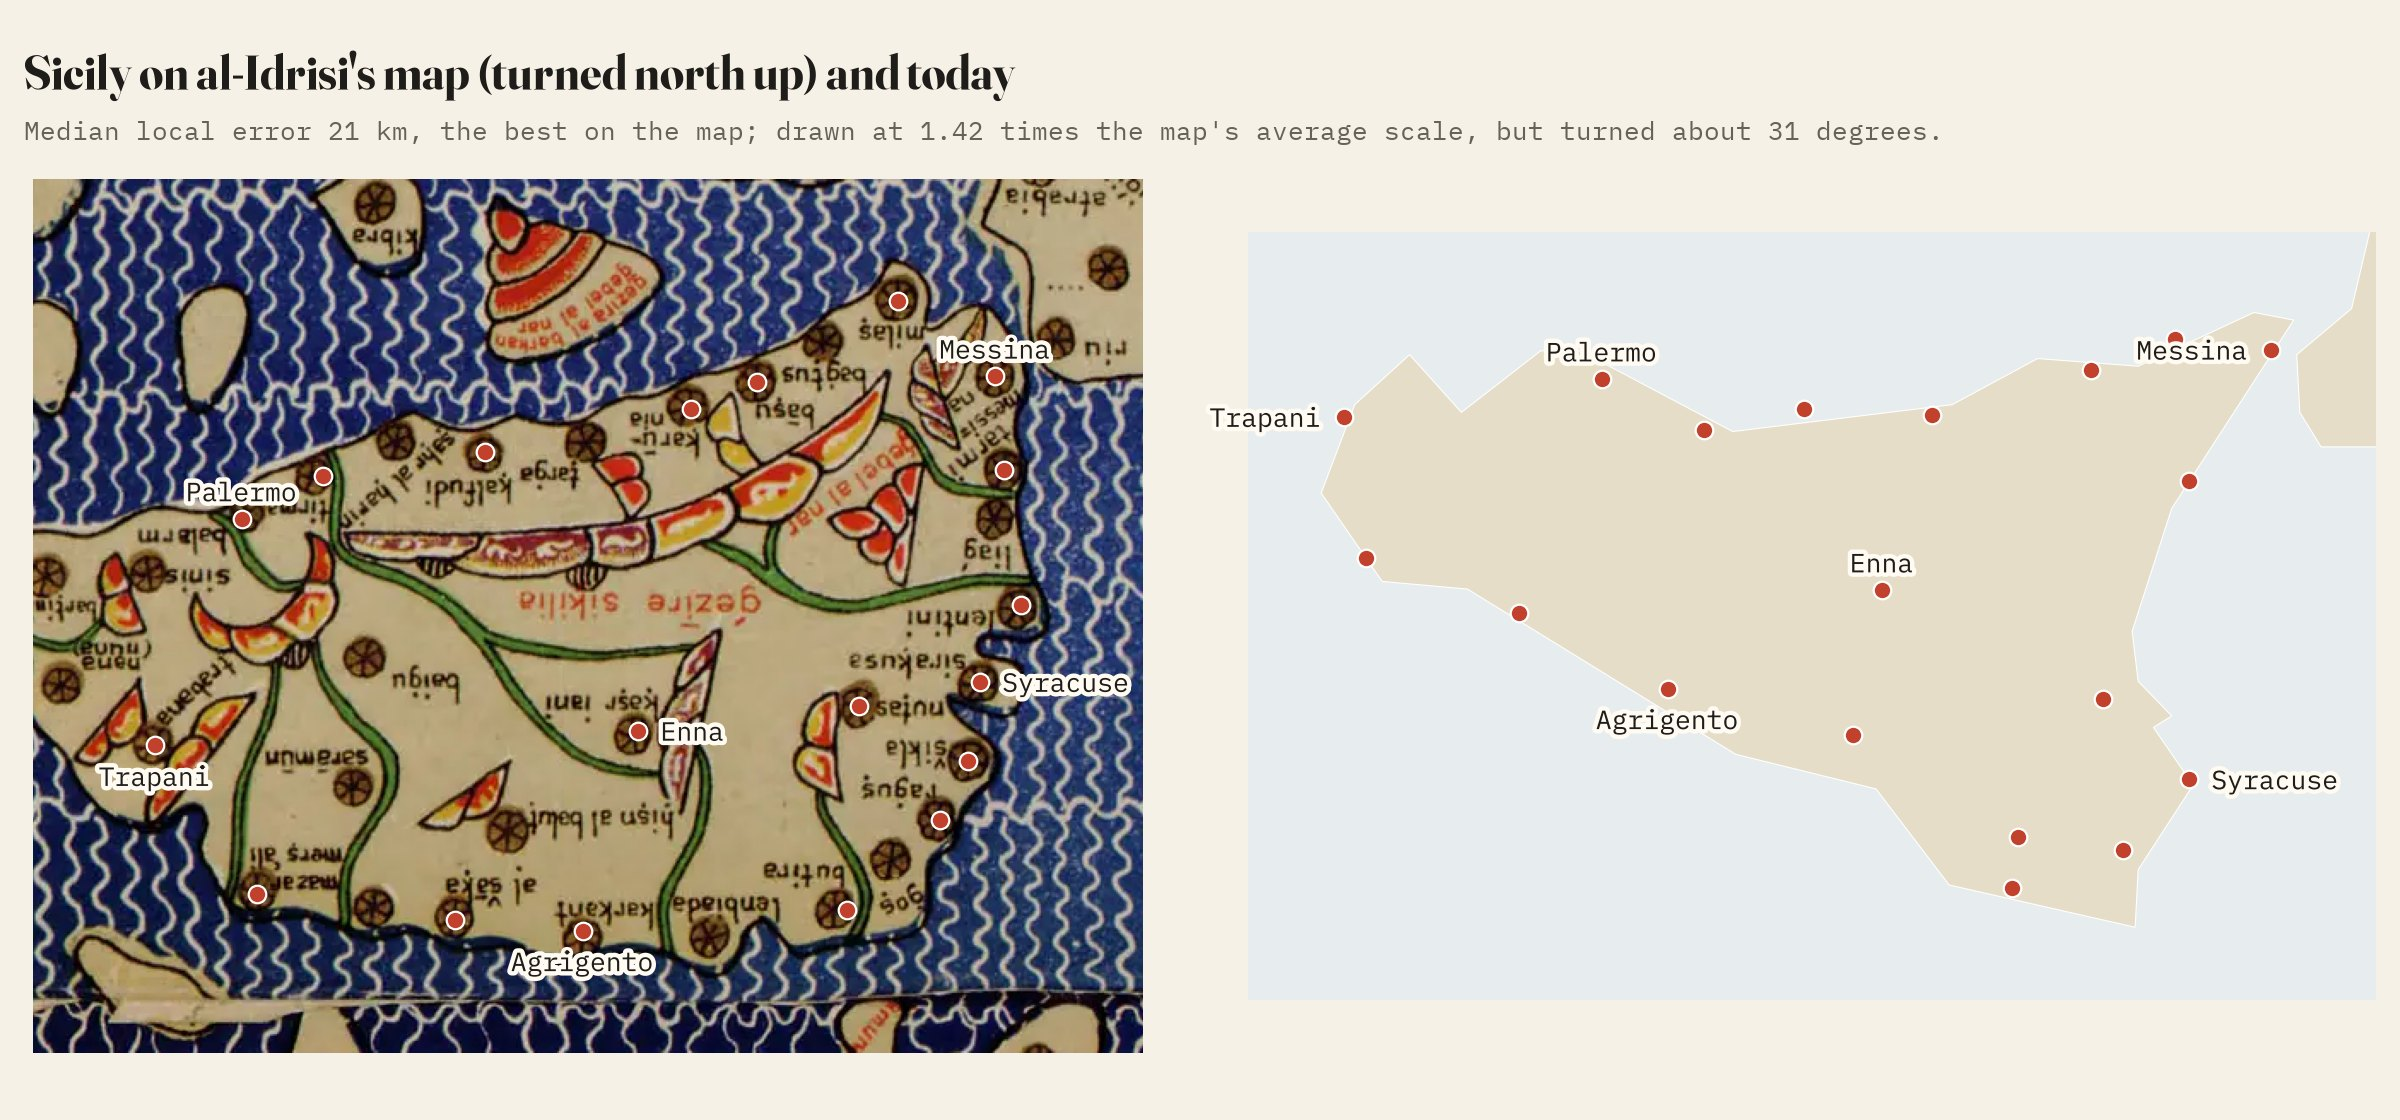
\includegraphics[width=\textwidth]{f_sicily.jpg}
\caption{Sicily on Miller's reconstruction (turned north up) and today.}\label{fig:sicily}\end{figure}

\subsection{The climates}
The median latitude of the towns rises without a break from climate to climate (Table~\ref{tab:climates}, Figure~\ref{fig:climates}). Every climate is drawn about the same height (a mean of 754 pixels), but the implied boundaries fall at 18.0, 28.6, 35.8, 40.4, 47.3 and 53.2 degrees north: the second climate spans 10.6 degrees and the third to sixth an average of 5.8. With these boundaries 74\% of towns lie in the climate their latitude would give and all lie within one. The first and seventh climates are thinly sampled (10 and 3 towns).

\begin{table}[tbp]\centering\small\caption{Towns by climate: number, minimum, median and maximum true latitude (degrees north), and the implied boundary with the next climate.}\label{tab:climates}\begin{tabular}{lrrrrr}\toprule Climate & Towns & Min & Median & Max & Boundary\\\midrule
I & 10 & 12.8 & 15.6 & 24.1 & 18.0\\
II & 36 & 14.8 & 25.3 & 34.6 & 28.6\\
III & 108 & 25.4 & 32.8 & 37.0 & 35.8\\
IV & 149 & 32.0 & 37.6 & 43.2 & 40.4\\
V & 80 & 37.8 & 41.3 & 47.3 & 47.3\\
VI & 45 & 41.0 & 48.4 & 52.5 & 53.2\\
VII & 3 & 51.1 & 53.2 & 53.6 & \\
\bottomrule\end{tabular}\end{table}

\begin{figure}[tbp]\centering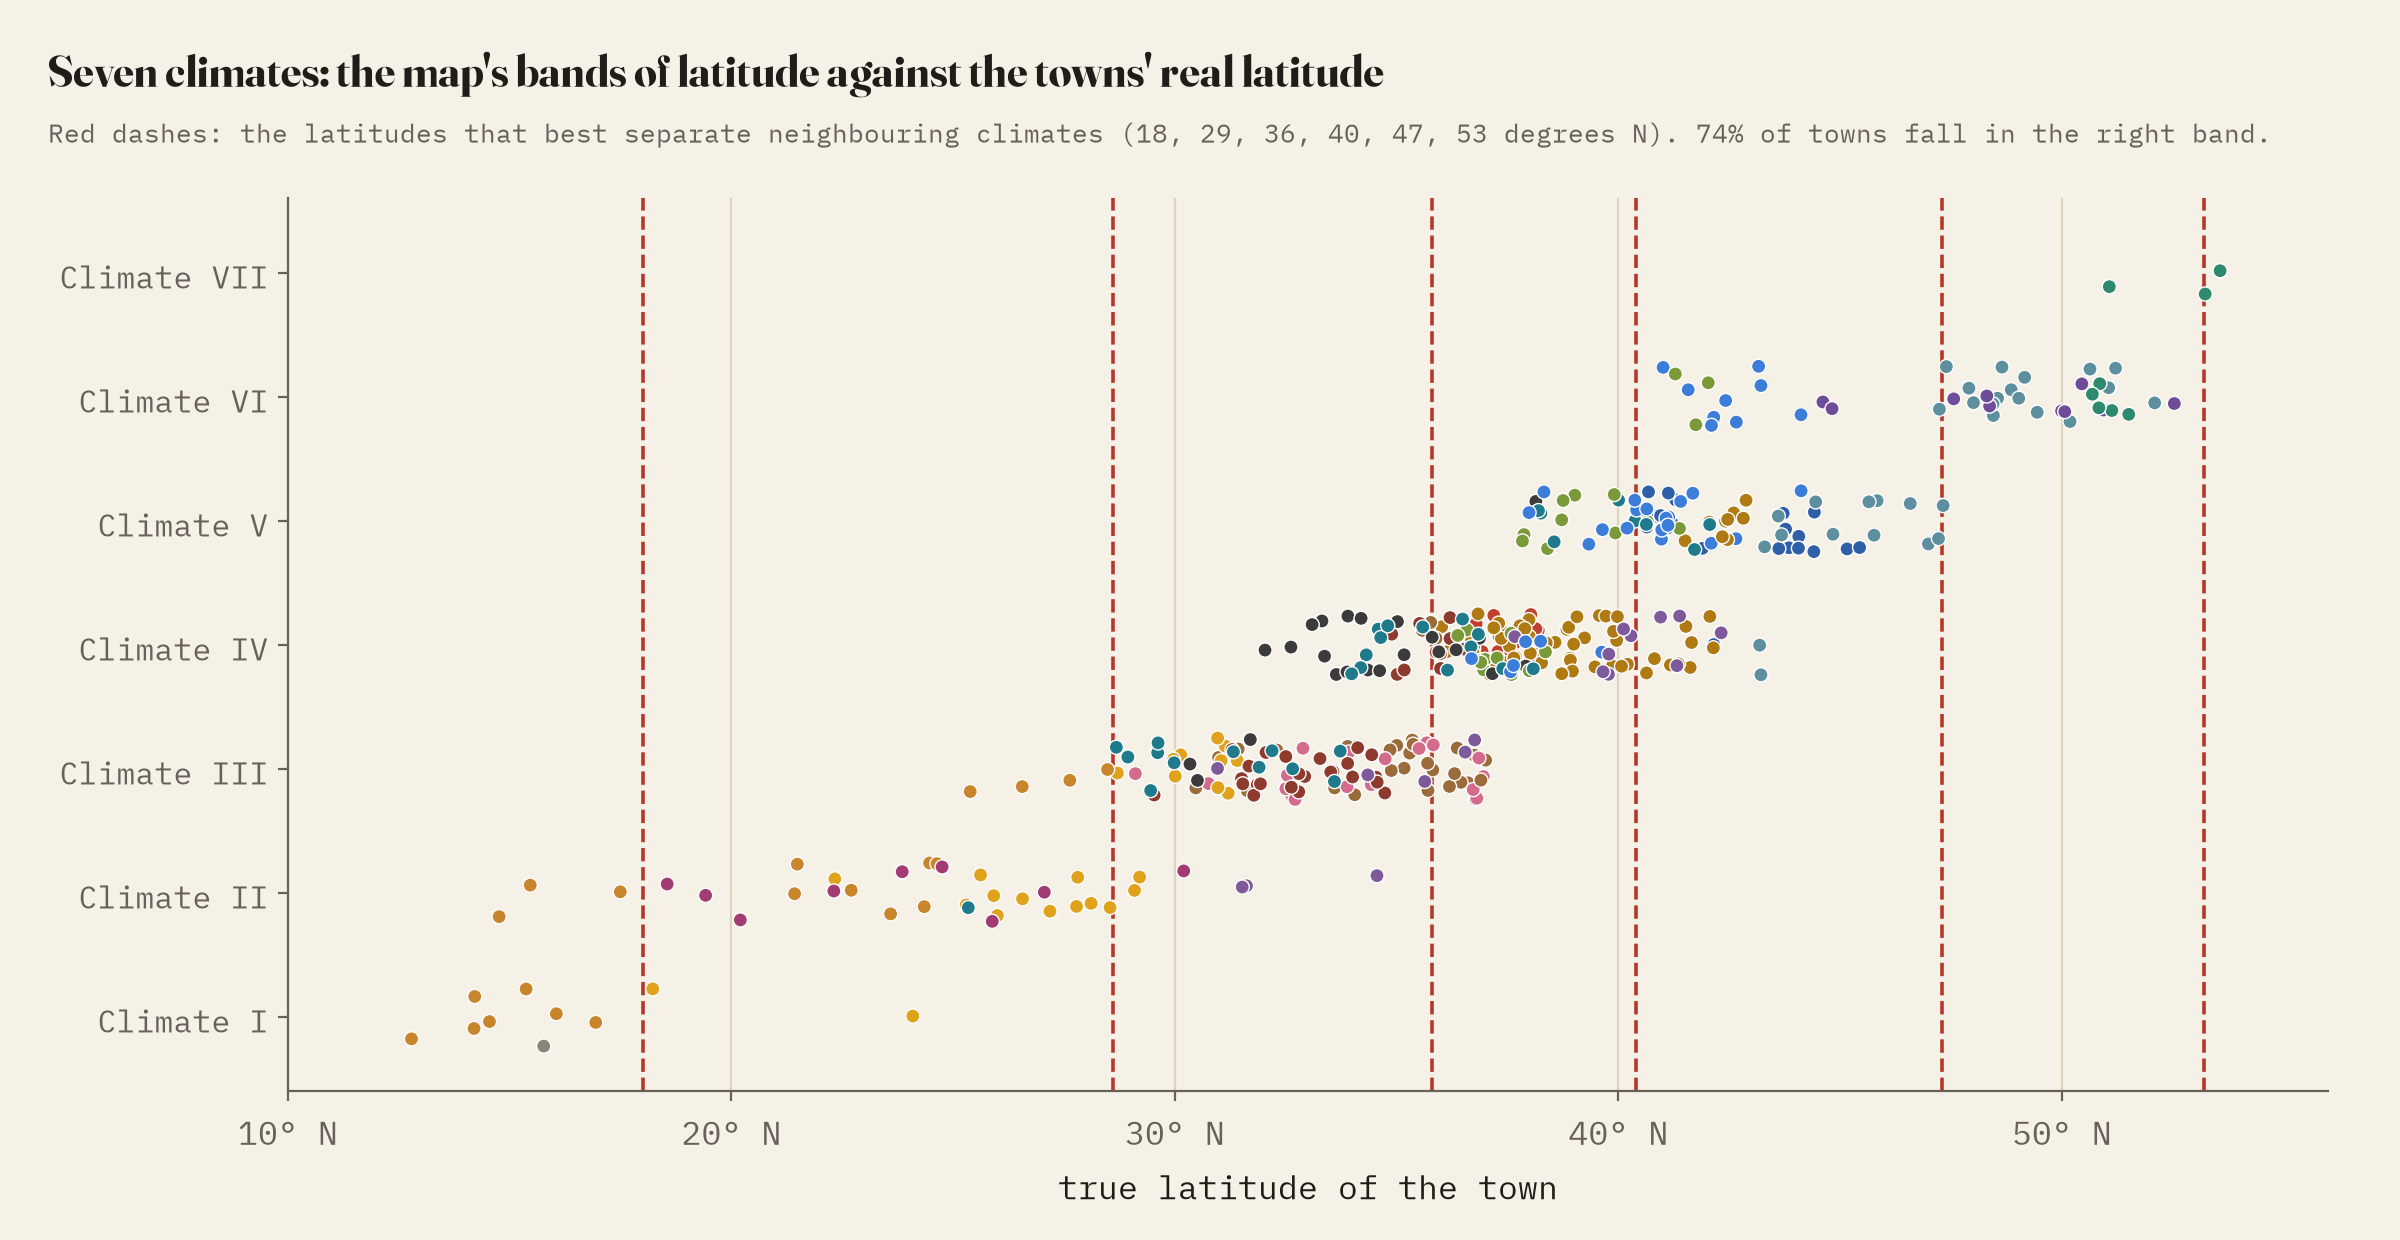
\includegraphics[width=\textwidth]{f_climates.png}
\caption{True latitude of the towns in each climate. Dashed lines: implied boundaries.}\label{fig:climates}\end{figure}

\subsection{The Nile}
The text places the source of the Nile in the Mountains of the Moon, ``whose beginning is sixteen degrees beyond the equinoctial line'' \citep{dozy}, and quotes Qudama that the river runs 5,654 miles from source to sea. On Miller's sheet the mountains sit only about 130 pixels beyond the equator line, about 0.17 of the height of a climate, so the map does not show sixteen degrees. At 1.92 to 2.0 km to the Arab mile, 5,654 miles is 10,900 to 11,300 km, against about 6,650 km for the real river. Along the river itself the map is good: under the global fit Aswan falls at 23.3 degrees north (really 24.1) and Alexandria at 32.5 (really 31.2), and Egypt's towns span 13.7 degrees of fitted latitude against 13.2 in reality.

\subsection{Britain}
I could read 8 English towns, too few for firm conclusions. They straddle the boundary between the sixth and seventh climates. Under the global fit their median latitude error is within a tenth of a degree, while they are displaced 2.3 degrees of longitude to the east, and the local fit is rotated about 37 degrees clockwise: Paris, 148 degrees from London in reality, is drawn at 191 degrees. Measured from Jerusalem, the English towns point the right way to within a median 12 degrees, against 8 for the British places on the Hereford map.

\subsection{Route distances}
The stated miles rise with the straight line distance (Spearman 0.89; Figure~\ref{fig:routes}), at a median of 1.42 km per mile (interquartile range 1.23 to 1.58). If the Arab mile is taken as 1.92 to 2.0 km, the stated road distances are 1.35 to 1.41 times the straight line, plausible for roads; alternatively the miles of these itineraries were shorter. A day stage is a median 36 km of straight line (interquartile range 30 to 43; Spearman 0.83), and in the 4 routes that give both, a day is about 25 miles. For the 18 routes in miles with both ends located on the map, map distance correlates more closely with the stated miles (Spearman 0.74) than with the true distance (0.48), consistent with a map compiled from itineraries, though the sample is small.

\begin{figure}[tbp]\centering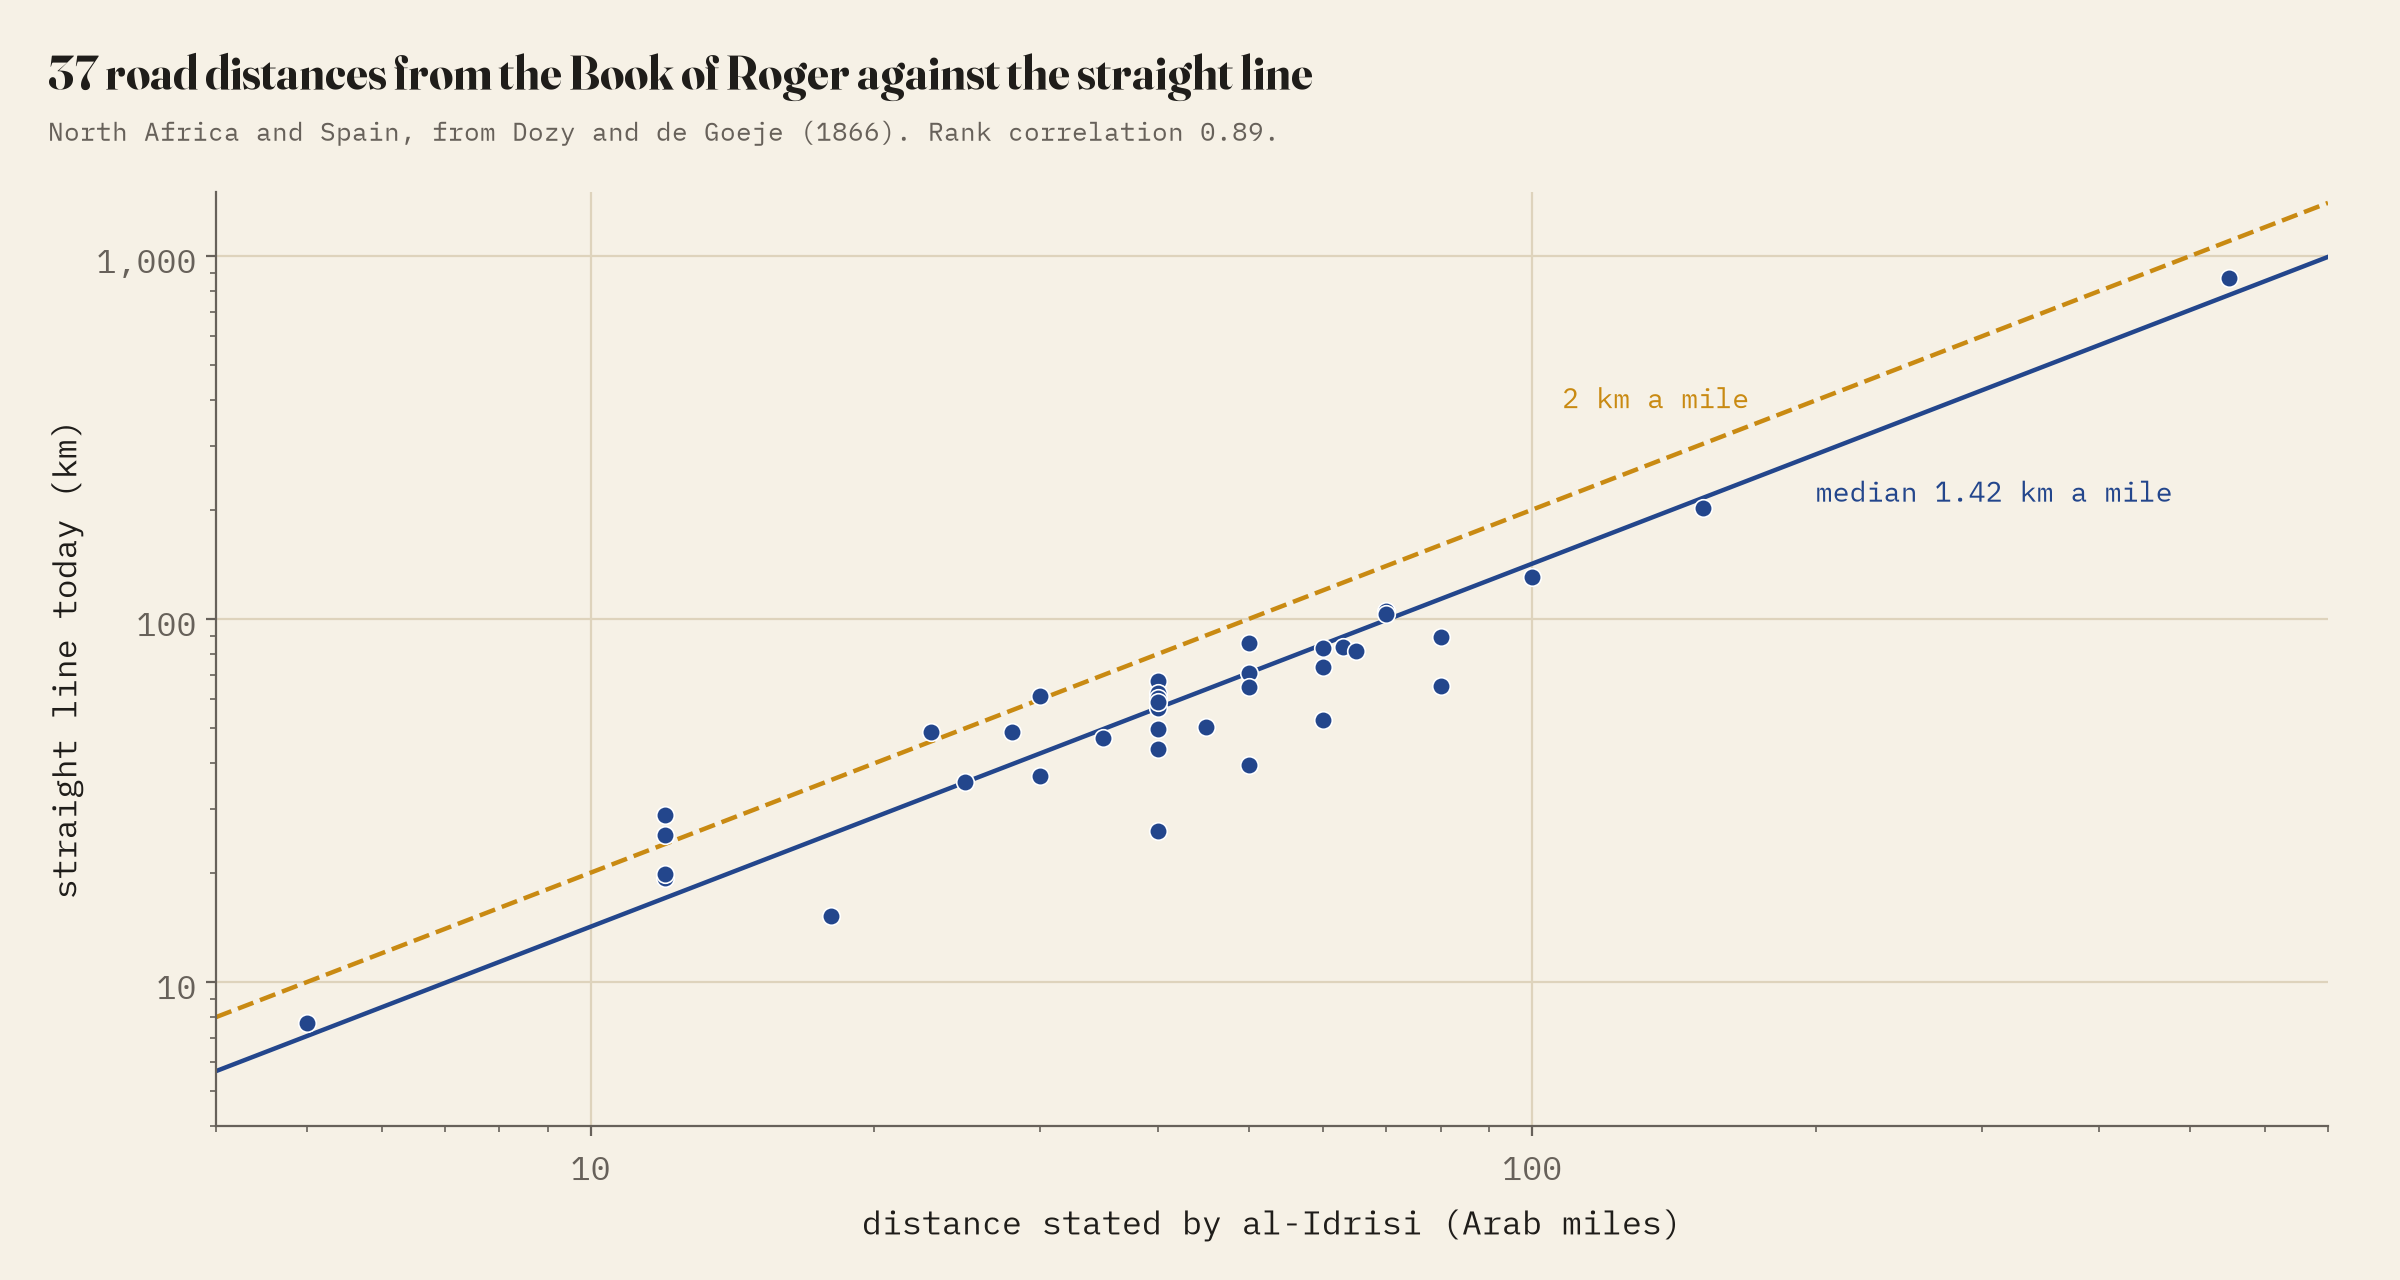
\includegraphics[width=\textwidth]{f_routes.png}
\caption{Distances stated in the Book of Roger (North Africa and Spain) against the great circle distance between the two places.}\label{fig:routes}\end{figure}

\subsection{Comparison with the Hereford Mappa Mundi}
On the Hereford study's measures (Figure~\ref{fig:compare}), the similarity fit about Jerusalem explains 0.94 of the spread of real positions on al-Idrisi's map against 0.84 on Hereford; the median displacement is 330 km against 516 km; the median bearing error from Jerusalem is 13 degrees against 19; and 99\% of places lie within 45 degrees against 81\%. Hereford draws the Holy Land at 4.5 times its average scale; al-Idrisi draws Syria and Palestine at 1.25.

\begin{figure}[tbp]\centering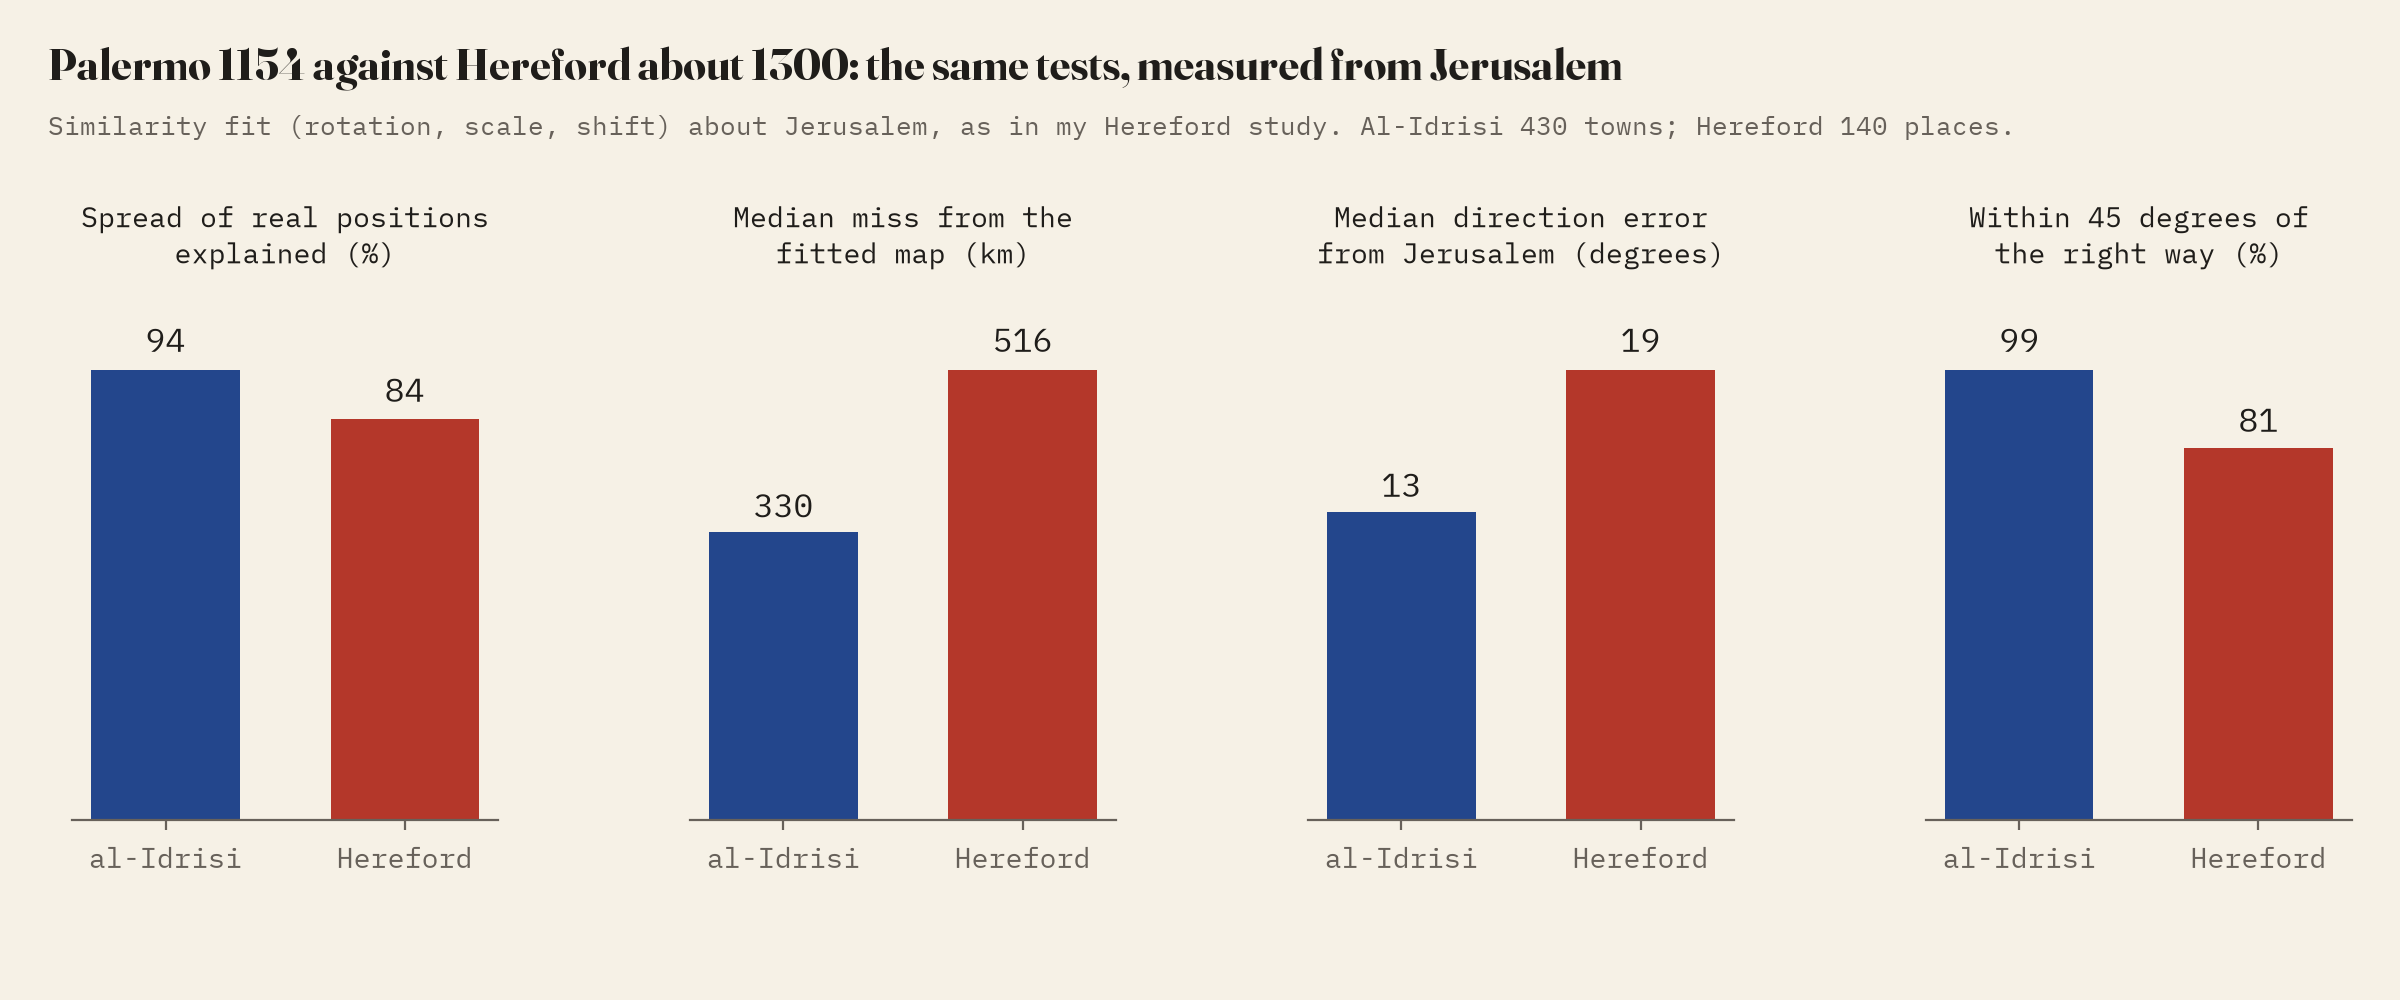
\includegraphics[width=\textwidth]{f_compare.png}
\caption{The same tests on al-Idrisi's map and on the Hereford Mappa Mundi.}\label{fig:compare}\end{figure}

\section{Limitations}
First, the map measured is Miller's reconstruction, which joins and redraws the section maps of the manuscripts; where his work departs from them, so do these measurements. Second, the sample is the legible, identifiable towns, about 431 of a much larger number of names; it favours well documented places, and it is thin in India and Central Asia, eastern Europe and Africa south of the Sahara (9, 10 and 1 towns). Third, the identifications and modern positions are mine; 85\% were confirmed in a gazetteer, and the rest are small places whose identification rests on the name and its position among its neighbours. Fourth, with clear readings only (362 towns) the median local error is 52 km and the median global residual 235 km, close to the full sample's. Fifth, the route distances come from one edition covering only North Africa and Spain, read from OCR and checked line by line, and the length of the Arab mile is uncertain. Sixth, the Hereford comparison sets a sample of medieval towns against a sample dominated by classical names; it compares the maps as sources of positions, not their makers' purposes.

\section{Conclusion}
Turned north up, al-Idrisi's map is a recognisable map of the Old World. It keeps directions between towns to a median of 10 degrees and keeps the shape of neighbourhoods best where its informants were most numerous: around the Mediterranean, and above all in Sicily, which it also draws larger than anywhere else. Its climates order the world by latitude while compressing the south and spreading out the populous middle latitudes. On the measures I applied to the Hereford Mappa Mundi, it is the more accurate map, as befits a geographer's survey compiled from travellers rather than a picture of Scripture and history; but both spend their space most generously on home.

\section*{Data and code availability}
The interactive comparison is at \url{https://maps.tristanhotham.com/idrisi/}. Data and code are at \url{https://github.com/Tristan-Hotham/idrisi} and archived with this paper at https://doi.org/10.5281/zenodo.23882607. Derived data are released under CC BY 4.0 and code under the MIT licence. Miller's reconstruction and the 1866 edition are in the public domain; al-Thurayya data are CC BY 4.0 and Pleiades data CC BY 3.0.

\section*{AI statement}
I wrote the text, with drafting and editing assistance from Claude (Anthropic), which also helped prepare the analysis code. I reviewed and checked all text and results.

\begin{thebibliography}{9}
\bibitem[Dozy and de Goeje(1866)]{dozy} Dozy, R. and de Goeje, M. J. (1866) \textit{Description de l'Afrique et de l'Espagne par Edrisi}. Leiden: Brill. Internet Archive scan, public domain. \url{https://archive.org/details/bub_gb_6EMNNqPF2zAC}
\bibitem[Hotham(2026)]{hereford} Hotham, T. (2026) The world according to the Hereford Mappa Mundi: a medieval map of the world set against a modern one. Zenodo. \url{https://doi.org/10.5281/zenodo.23878612}
\bibitem[Miller(1928)]{miller1928} Miller, K. (1928) \textit{Charta Rogeriana: Weltkarte des Idrisi vom Jahr 1154 n. Ch.} Stuttgart. Wikimedia Commons, public domain. \url{https://commons.wikimedia.org/wiki/File:Tabula_Rogeriana_1929_copy_by_Konrad_Miller.jpg}
\bibitem[Natural Earth(2026)]{naturalearth} Natural Earth (2026) Admin 0 countries and populated places, 1:50m and 1:10m. Public domain. \url{https://www.naturalearthdata.com/}
\bibitem[Pleiades(2026)]{pleiades} Bagnall, R. et al., eds. (2026) Pleiades: a gazetteer of past places, version 4.1. CC BY 3.0. \url{https://pleiades.stoa.org/}
\bibitem[Seydi and Romanov(2026)]{thurayya} Seydi, M. and Romanov, M. (2026) al-Thurayya Gazetteer, places and routes of the early Islamic world, from G. Cornu (1983) \textit{Atlas du monde arabo-islamique}. CC BY 4.0. \url{https://github.com/althurayya/althurayya.github.io}
\end{thebibliography}

\clearpage
\appendix
\section{The route distances}
{\footnotesize\begin{longtable}{p{4.2cm}p{4.2cm}rrrr}\caption{Distances stated by al-Idrisi in Dozy and de Goeje (1866): miles, day stages, great circle distance today (km) and the line of the Internet Archive text.}\label{tab:routes}\\\toprule From & To & Miles & Days & km & Line\\\midrule\endfirsthead\toprule From & To & Miles & Days & km & Line\\\midrule\endhead
Fez & Meknes & 40 &  & 57 & 5062\\
Aghmat & Marrakesh & 12 &  & 29 & 4623\\
Jijel & Bejaia & 30 &  & 61 & 6297\\
Algiers & Tamenfoust & 18 &  & 15 & 5859\\
Bizerte & Tabarka & 70 &  & 105 & 7275\\
Monastir & Mahdia & 30 &  & 37 & 8024\\
Tocra & Ptolemais (Tolmeita) & 50 &  & 40 & 8513\\
Barca (al-Marj) & Ajdabiya & 152 & 6 & 202 & 8392\\
Barca (al-Marj) & Alexandria & 550 & 21 & 870 & 8394\\
Rosetta (Rashid) & Alexandria & 60 &  & 53 & 10097\\
Cadiz & Tarifa & 63 &  & 84 & 11186\\
Faro (Santa Maria) & Silves & 28 &  & 49 & 11223\\
Guadalajara & Medinaceli & 50 &  & 86 & 11809\\
Daroca & Zaragoza & 60 &  & 74 & 11850\\
Calatayud & Zaragoza & 50 &  & 71 & 11852\\
Zaragoza & Huesca & 40 &  & 68 & 11881\\
Huesca & Lleida & 70 &  & 103 & 11883\\
Mequinenza & Tortosa & 50 & 2 & 65 & 11890\\
Tarragona & Barcelona & 60 &  & 83 & 11913\\
Alzira & Xativa & 12 &  & 19 & 11982\\
Valencia & Denia & 65 &  & 82 & 11992\\
Valencia & Cullera & 25 &  & 36 & 11994\\
Xativa & Bocairent & 40 &  & 26 & 12026\\
Bocairent & Denia & 40 &  & 63 & 12035\\
Orihuela & Murcia & 12 &  & 20 & 12074\\
Cartagena & Murcia & 40 &  & 44 & 12153\\
Lorca & Murcia & 40 &  & 61 & 12299\\
Almunecar & Granada & 40 &  & 50 & 12487\\
Granada & Loja & 23 &  & 49 & 12868\\
Almunecar & Malaga & 80 &  & 65 & 12872\\
Malaga & Granada & 80 &  & 89 & 12890\\
Lucena & Cordoba & 40 &  & 59 & 12992\\
Ecija & Cordoba & 35 &  & 47 & 13012\\
Ecija & Carmona & 45 &  & 50 & 13020\\
Jerez de la Frontera & Isla de Leon (San Fernando) & 12 &  & 25 & 13049\\
Cordoba & Madinat al-Zahra & 5 &  & 8 & 13475\\
Cordoba & Granada & 100 & 4 & 131 & 13655\\
Sale & Fez &  & 4 & 168 & 4995\\
Fez & Sijilmasa &  & 13 & 317 & 5042\\
Tlemcen & Tahert (Tiaret) &  & 4 & 246 & 5683\\
Tenes & Miliana &  & 2 & 86 & 5798\\
M'Sila & Tobna &  & 2 & 83 & 6116\\
Tobna & Bejaia &  & 6 & 158 & 6130\\
Constantine & Bejaia &  & 6 & 143 & 6295\\
Collo & Constantine &  & 2 & 71 & 6406\\
Setif & Constantine &  & 4 & 110 & 6418\\
Sfax & Gafsa &  & 3 & 184 & 6911\\
Sfax & Mahdia &  & 2 & 89 & 6934\\
Kairouan & Tunis &  & 2 & 126 & 7097\\
Barca (al-Marj) & Awjila &  & 10 & 380 & 8390\\
Fustat (Old Cairo) & Oxyrhynchus (al-Bahnasa) &  & 7 & 172 & 10130\\
Fustat (Old Cairo) & Aswan &  & 26 & 678 & 3886\\
Algeciras & Seville &  & 5 & 148 & 11025\\
Silves & Badajoz &  & 3 & 228 & 11252\\
Evora & Badajoz &  & 2 & 88 & 11332\\
Badajoz & Seville &  & 6 & 187 & 11356\\
Badajoz & Cordoba &  & 6 & 220 & 11359\\
Merida & Alcantara &  & 2 & 101 & 11451\\
Santarem & Badajoz &  & 4 & 153 & 11631\\
Valencia & Zaragoza &  & 9 & 246 & 11969\\
Murcia & Valencia &  & 5 & 178 & 12180\\
Murcia & Almeria &  & 5 & 174 & 12182\\
Cordoba & Almeria &  & 8 & 236 & 13489\\
\bottomrule\end{longtable}}

\section{The located towns}
{\footnotesize\setlength{\tabcolsep}{4pt}\begin{longtable}{p{4.6cm}p{3.0cm}p{3.6cm}llr}\caption{The 431 located towns: identification, Miller's transcription, region, climate, my confidence in the reading, and local error (km).}\label{tab:located}\\\toprule Town & On the map & Region & Clim. & Reading & Local\\\midrule\endfirsthead\toprule Town & On the map & Region & Clim. & Reading & Local\\\midrule\endhead
Adana & adana & Anatolia & IV & high & 81\\
Ahlat & halat & Anatolia & V & high & 88\\
Amasra (Amastris) & samastru & Anatolia & VI & high & 52\\
Amasya & amasia & Anatolia & V & high & 137\\
Amorium & amuria & Anatolia & V & high & 62\\
Anazarbus (Ayn Zarba) & ain zarba & Anatolia & IV & high & 77\\
Ankara & ankira & Anatolia & V & medium & 255\\
Antalya & antalia & Anatolia & IV & high & 263\\
Bitlis & bidlis & Anatolia & V & high & 53\\
Erzurum (Qaliqala) & kalikala & Anatolia & V & high & 166\\
Iskenderun & iskanderuna & Anatolia & IV & high & 93\\
Kahramanmaras & maras & Anatolia & IV & high & 93\\
Karadeniz Eregli (Heraclea Pontica) & heraklia & Anatolia & VI & high & 67\\
Kastamonu & kastamuni & Anatolia & V & high & 159\\
Kayseri & kaisaria & Anatolia & V & high & 233\\
Konya & kunia & Anatolia & V & high & 203\\
Laodicea on the Lycus & ladikia & Anatolia & V & medium & 152\\
Malatya & malatia & Anatolia & IV & high & 87\\
Mopsuestia (al-Massisa) & al masisa & Anatolia & IV & high & 71\\
Samosata (Samsat) & samsat & Anatolia & IV & high & 38\\
Silifke (Seleucia) & selukia & Anatolia & IV & high & 60\\
Sinop & sinuboli & Anatolia & VI & high & 126\\
Tarsus & tarsus & Anatolia & IV & high & 65\\
al-Hadath & al hadit & Anatolia & IV & high & 57\\
Aden & aden & Arabia & I & high & 156\\
Dhamar & damar & Arabia & I & high & 134\\
Hajr al-Yamama (Riyadh) & hagar al iemama & Arabia & II & medium & 165\\
Jeddah & gidda & Arabia & II & high & 21\\
Madyan (al-Bad) & madjan & Arabia & III & medium & 138\\
Marib & marib & Arabia & II & high & 181\\
Mecca & mekka & Arabia & II & high & 53\\
Medina (Yathrib) & iatrib & Arabia & II & high & 65\\
Muscat & maskat & Arabia & II & high & 338\\
Najran & negran & Arabia & II & high & 135\\
Qatif & al katif & Arabia & III & high & 236\\
Saada & saada & Arabia & I & high & 134\\
Sanaa & sanaa & Arabia & I & high & 101\\
Sohar & sohar & Arabia & II & high & 339\\
Tarim & tarim & Arabia & I & high & 314\\
Tayma & teima & Arabia & III & high & 328\\
Zabid & zabid & Arabia & I & high & 80\\
Zafar (Yemen) & tafar & Arabia & I & high & 187\\
al-Ahsa (Hofuf) & al ahsa & Arabia & III & high & 205\\
al-Juhfa & al gofa & Arabia & II & medium & 89\\
al-Shihr & madina al sihr & Arabia & II & high & 208\\
Akhsikath & ahsikat & Central Asia and Afghanistan & IV & high & 58\\
Andarab & indarab & Central Asia and Afghanistan & III & high & 250\\
Balkh & balh & Central Asia and Afghanistan & III & high & 84\\
Bost (Lashkar Gah) & bost & Central Asia and Afghanistan & II & high & 288\\
Bukhara & buhari & Central Asia and Afghanistan & IV & high & 92\\
Hazarasp & hazarasb & Central Asia and Afghanistan & IV & high & 163\\
Herat & herat & Central Asia and Afghanistan & III & medium & 280\\
Jizzakh & gizak & Central Asia and Afghanistan & IV & medium & 216\\
Kabul & kabul & Central Asia and Afghanistan & II & medium & 78\\
Kandahar & al kandahar & Central Asia and Afghanistan & II & medium & 586\\
Kath (Khwarazm) & kat & Central Asia and Afghanistan & IV & medium & 47\\
Khujand & hogand & Central Asia and Afghanistan & IV & high & 48\\
Kunya-Urgench (Gurganj) & gorgania & Central Asia and Afghanistan & IV & high & 163\\
Merv & maru al sahgan & Central Asia and Afghanistan & IV & high & 164\\
Paykand & baikand & Central Asia and Afghanistan & IV & high & 24\\
Samarkand & samarkand & Central Asia and Afghanistan & IV & medium & 48\\
Sarakhs & sarahs & Central Asia and Afghanistan & III & high & 111\\
Zaranj & zarang & Central Asia and Afghanistan & III & high & 210\\
Augsburg & auzburk & Central and Eastern Europe & VI & high & 206\\
Basel & bazla & Central and Eastern Europe & VI & high & 105\\
Belgrade & belgraba & Central and Eastern Europe & VI & high & 521\\
Chersonesus (Kherson) & karsuna & Central and Eastern Europe & VI & medium & 217\\
Cologne & kolunia & Central and Eastern Europe & VI & high & 80\\
Gniezno & genasia & Central and Eastern Europe & VI & medium & 566\\
Krakow & akrakal & Central and Eastern Europe & VI & medium & 300\\
Kyiv & kiau & Central and Eastern Europe & VI & medium & 657\\
Mainz & maiansa & Central and Eastern Europe & VI & high & 164\\
Nitra & neitram & Central and Eastern Europe & VI & high & 66\\
Akhmim & ahmim & Egypt and Nubia & II & high & 70\\
Alexandria & al iskanderia & Egypt and Nubia & III & high & 21\\
Antinoe (Ansina) & ansana & Egypt and Nubia & II & high & 33\\
Armant & arment & Egypt and Nubia & II & high & 111\\
Aswan & asuan & Egypt and Nubia & I & high & 71\\
Asyut & assiut & Egypt and Nubia & II & high & 208\\
Aydhab & aidab & Egypt and Nubia & II & high & 161\\
El Arish & al aris & Egypt and Nubia & III & high & 34\\
El Mahalla el Kubra & al mahalla & Egypt and Nubia & III & high & 23\\
Esna & asnah & Egypt and Nubia & II & high & 72\\
Fustat (Old Cairo) & misr & Egypt and Nubia & III & high & 17\\
Heliopolis (Ain Shams) & ain sams & Egypt and Nubia & III & high & 72\\
Hermopolis (al-Ashmunayn) & asmun & Egypt and Nubia & II & high & 61\\
Ihnasya (Ahnas) & ahnas & Egypt and Nubia & II & high & 64\\
Minya & miniat ibn al hasib & Egypt and Nubia & II & medium & 56\\
Old Dongola & donkla & Egypt and Nubia & I & medium & 657\\
Oxyrhynchus (al-Bahnasa) & al bahnasa & Egypt and Nubia & II & high & 27\\
Pelusium (al-Farama) & al farama & Egypt and Nubia & III & high & 61\\
Pharan (Feiran) & faran & Egypt and Nubia & III & medium & 101\\
Qift & kaft & Egypt and Nubia & II & high & 130\\
Qus & kus & Egypt and Nubia & II & high & 87\\
Rosetta (Rashid) & rasid & Egypt and Nubia & III & high & 12\\
Samannud & samnud & Egypt and Nubia & III & medium & 11\\
Siwa & santaria & Egypt and Nubia & II & high & 29\\
Suez (al-Qulzum) & al kolzum & Egypt and Nubia & III & high & 60\\
Dover & dobrs & England & VI & high & 45\\
Grimsby & agrims & England & VII & high & 153\\
Hastings & hastinks & England & VI & high & 10\\
Lincoln & nikula & England & VII & medium & 115\\
London & londr & England & VI & high & 55\\
Salisbury & salaberis & England & VII & high & 170\\
Shoreham-by-Sea & sorham & England & VI & medium & 21\\
Wareham & garham & England & VI & medium & 71\\
Angouleme & ankolazma & France and the Low Countries & V & medium & 24\\
Besancon & besanzun & France and the Low Countries & VI & high & 187\\
Bordeaux & bordal & France and the Low Countries & V & high & 79\\
Bruges & abrugs & France and the Low Countries & VI & high & 35\\
Cahors & kaurs & France and the Low Countries & V & medium & 160\\
Carcassonne & karkasuna & France and the Low Countries & IV & high & 55\\
Chartres & gartas & France and the Low Countries & VI & high & 43\\
Dijon & digun & France and the Low Countries & V & high & 73\\
Dinan & dinam & France and the Low Countries & VI & high & 52\\
Dol-de-Bretagne & dul & France and the Low Countries & VI & high & 43\\
Evreux & abraus & France and the Low Countries & VI & medium & 59\\
Ghent & kent & France and the Low Countries & VI & high & 71\\
Le Mans & al mais & France and the Low Countries & VI & medium & 81\\
Liege & liaga & France and the Low Countries & VI & high & 29\\
Limoges & limuges & France and the Low Countries & V & high & 129\\
Lyon & liun & France and the Low Countries & V & high & 78\\
Marseille & masilia & France and the Low Countries & V & high & 69\\
Nantes & nanitas & France and the Low Countries & V & high & 70\\
Narbonne & arbuna & France and the Low Countries & IV & high & 97\\
Nevers & nifaras & France and the Low Countries & V & medium & 53\\
Orleans & arlians & France and the Low Countries & VI & high & 28\\
Paris & abariz & France and the Low Countries & VI & high & 10\\
Poitiers & bataras & France and the Low Countries & V & medium & 83\\
Quimper (Saint-Corentin) & kerenbin sant karnin & France and the Low Countries & VI & medium & 8\\
Rouen & ratumagus & France and the Low Countries & VI & high & 53\\
Saint-Gilles & sant gili & France and the Low Countries & V & high & 30\\
Saint-Malo & sant mahlu & France and the Low Countries & VI & high & 54\\
Saint-Valery-sur-Somme & sant ualeri & France and the Low Countries & VI & medium & 17\\
Toulouse & tolusa & France and the Low Countries & V & high & 85\\
Tours & tars & France and the Low Countries & VI & medium & 80\\
Utrecht & astrik & France and the Low Countries & VI & medium & 16\\
Verdun & berdun & France and the Low Countries & VI & high & 77\\
Abydos (Dardanelles) & abidus & Greece and the Balkans & V & high & 17\\
Ahtopol (Agathopolis) & agatubolus & Greece and the Balkans & VI & high & 50\\
Argos & argu & Greece and the Balkans & IV & high & 22\\
Athens & atina & Greece and the Balkans & V & high & 156\\
Bar (Antivari) & antibra & Greece and the Balkans & V & high & 105\\
Constantinople (Istanbul) & al kostantina & Greece and the Balkans & VI & high & 119\\
Corfu & marnisa (kurfus) & Greece and the Balkans & IV & high & 187\\
Corinth & korint & Greece and the Balkans & IV & high & 29\\
Demetrias & dimitriana & Greece and the Balkans & V & medium & 44\\
Dubrovnik (Ragusa) & ragusa & Greece and the Balkans & V & high & 86\\
Edirne (Adrianople) & adirnuboli & Greece and the Balkans & V & high & 77\\
Gallipoli (Gelibolu) & kalibolu & Greece and the Balkans & V & high & 45\\
Kitros (Pydna) & kitrus & Greece and the Balkans & V & medium & 111\\
Larissa & larisa & Greece and the Balkans & V & medium & 147\\
Luleburgaz (Arcadiopolis) & arkadiuboli & Greece and the Balkans & V & high & 16\\
Marmara Ereglisi (Heraclea) & heraklia & Greece and the Balkans & V & high & 20\\
Monemvasia & maliasa & Greece and the Balkans & IV & high & 83\\
Nafplio & anubali & Greece and the Balkans & IV & high & 27\\
Nesebar (Mesembria) & mesinus & Greece and the Balkans & VI & medium & 84\\
Ohrid & ahrida & Greece and the Balkans & V & high & 40\\
Patras & bras & Greece and the Balkans & IV & medium & 158\\
Plovdiv (Philippopolis) & filibus & Greece and the Balkans & VI & high & 167\\
Preslav & barsklafa & Greece and the Balkans & VI & medium & 78\\
Silistra (Dristra) & darsira & Greece and the Balkans & VI & medium & 147\\
Silivri (Selymbria) & salimria & Greece and the Balkans & V & high & 40\\
Sozopol & sizuboli & Greece and the Balkans & VI & high & 42\\
Tekirdag (Rodosto) & rudostu & Greece and the Balkans & V & high & 28\\
Thebes & astifas & Greece and the Balkans & V & high & 69\\
Thessaloniki & salunik & Greece and the Balkans & V & high & 141\\
Varna & barnas & Greece and the Balkans & VI & high & 168\\
Vize & bizi & Greece and the Balkans & VI & high & 55\\
Zadar & gadra & Greece and the Balkans & V & medium & 76\\
Alcacer do Sal & al kasr & Iberia & IV & high & 105\\
Alcantara & al kantara al sif & Iberia & IV & high & 36\\
Algeciras & al gezira & Iberia & IV & high & 26\\
Alicante & lekant & Iberia & IV & high & 39\\
Almeria & al meria & Iberia & IV & high & 37\\
Almunecar & al monkab & Iberia & IV & high & 21\\
Archidona & arsiduna & Iberia & IV & high & 3\\
Astorga & astorka & Iberia & V & high & 17\\
Badajoz & batalius & Iberia & IV & high & 73\\
Baeza & baisa & Iberia & IV & high & 53\\
Baza & basta & Iberia & IV & high & 31\\
Burgos & burgas & Iberia & V & high & 36\\
Burriana & boriana & Iberia & IV & high & 27\\
Calatayud & kalaat aiub & Iberia & IV & high & 55\\
Calatrava la Vieja & kalaat rabah & Iberia & IV & high & 36\\
Cartagena & kartagena & Iberia & IV & high & 77\\
Coimbra & kalimria & Iberia & IV & high & 67\\
Cordoba & kortoba & Iberia & IV & medium & 22\\
Coria & koria & Iberia & IV & high & 46\\
Cuenca & kuenka & Iberia & IV & high & 65\\
Denia & dania & Iberia & IV & high & 11\\
Ecija & asiha & Iberia & IV & high & 44\\
Elche & els & Iberia & IV & high & 8\\
Evora & iabara & Iberia & IV & high & 17\\
Fraga & afraga & Iberia & IV & high & 32\\
Granada & al granata & Iberia & IV & high & 8\\
Guadalajara & uadi al hagara & Iberia & IV & medium & 40\\
Guadix & uadias & Iberia & IV & high & 14\\
Huesca & ueska & Iberia & IV & high & 92\\
Ibiza & iabesa & Iberia & IV & high & 52\\
Jaen & gijan & Iberia & IV & high & 49\\
Jerez de la Frontera & seris & Iberia & IV & high & 25\\
Leon & liun & Iberia & V & high & 71\\
Lisbon & asbuna & Iberia & IV & high & 20\\
Lleida & lerida & Iberia & IV & high & 69\\
Logrono & kastila (logrono) & Iberia & V & medium & 56\\
Lorca & lurka & Iberia & IV & high & 56\\
Majorca (Palma) & maiorka & Iberia & IV & high & 79\\
Malaga & malaka & Iberia & IV & medium & 36\\
Medellin & medellin & Iberia & IV & high & 44\\
Medinaceli & medinat salim & Iberia & IV & high & 27\\
Merida & merida & Iberia & IV & medium & 71\\
Mertola & martala & Iberia & IV & high & 70\\
Murcia & mursia & Iberia & IV & high & 28\\
Najera & nagra & Iberia & V & high & 30\\
Niebla & libla & Iberia & IV & high & 19\\
Osuna & osuna & Iberia & IV & high & 39\\
Pamplona & banbluna & Iberia & V & high & 47\\
Santarem & santarin & Iberia & IV & high & 85\\
Santiago de Compostela & sant iakub & Iberia & V & high & 26\\
Seville & isbilia & Iberia & IV & high & 34\\
Silves & silb & Iberia & IV & medium & 95\\
Talavera de la Reina & talabera & Iberia & IV & high & 87\\
Tarifa & tarif & Iberia & IV & high & 23\\
Toledo & tolaitola & Iberia & IV & high & 28\\
Tortosa & tartusa & Iberia & IV & high & 37\\
Tudela & tutila & Iberia & IV & high & 86\\
Tui & duia & Iberia & V & medium & 68\\
Ubeda & abda & Iberia & IV & high & 34\\
Ucles & uklis & Iberia & IV & high & 38\\
Valencia & balinsia & Iberia & IV & high & 31\\
Xativa & satiba & Iberia & IV & high & 74\\
Zamora & samura & Iberia & V & high & 104\\
Zaragoza & sarakostia & Iberia & IV & high & 30\\
Abhar & abhar & Iran and the Caucasus & IV & high & 41\\
Ahvaz & al ahuaz & Iran and the Caucasus & III & high & 81\\
Ardabil & ardabil & Iran and the Caucasus & V & high & 177\\
Barda & bardaa & Iran and the Caucasus & V & high & 93\\
Bastam & bastam & Iran and the Caucasus & IV & high & 14\\
Derbent & bab al abuab & Iran and the Caucasus & V & high & 305\\
Dinawar & dainur & Iran and the Caucasus & IV & high & 76\\
Dvin & dabil & Iran and the Caucasus & V & high & 106\\
Fasa & fasa & Iran and the Caucasus & III & high & 285\\
Gorgan (Astarabad) & asterabad & Iran and the Caucasus & IV & high & 210\\
Hamadan & hamadan & Iran and the Caucasus & IV & high & 149\\
Isfahan & isbahan & Iran and the Caucasus & III & high & 36\\
Istakhr & istahr & Iran and the Caucasus & III & high & 47\\
Jiroft & giraft & Iran and the Caucasus & III & high & 47\\
Kashan & kasan & Iran and the Caucasus & IV & high & 38\\
Kazerun & kazerun & Iran and the Caucasus & III & high & 92\\
Kermanshah (Qirmisin) & karmasin & Iran and the Caucasus & IV & high & 27\\
Khoy & hui & Iran and the Caucasus & V & high & 105\\
Maragheh & al maraga & Iran and the Caucasus & IV & high & 39\\
Nahavand & nahauand & Iran and the Caucasus & IV & high & 4\\
Qayen & kain & Iran and the Caucasus & III & high & 111\\
Qom & kum & Iran and the Caucasus & IV & high & 97\\
Rayy & al rai & Iran and the Caucasus & IV & high & 54\\
Salmas & salmas & Iran and the Caucasus & V & high & 111\\
Shamakhi & al samahia & Iran and the Caucasus & V & high & 160\\
Shiraz & siraz & Iran and the Caucasus & III & high & 30\\
Sirjan & al sirgan & Iran and the Caucasus & III & high & 58\\
Susa (Shush) & sus & Iran and the Caucasus & III & high & 20\\
Tabas & al tabein & Iran and the Caucasus & III & medium & 206\\
Tabriz & tabriz & Iran and the Caucasus & IV & high & 141\\
Tbilisi & tiflis & Iran and the Caucasus & V & high & 81\\
Tiz & al taiza & Iran and the Caucasus & II & medium & 116\\
Yazd & iazd & Iran and the Caucasus & III & high & 37\\
Zanjan & zangan & Iran and the Caucasus & IV & high & 65\\
Abadan & abadan & Iraq and the Jazira & III & high & 49\\
Baghdad & bagdad & Iraq and the Jazira & IV & high & 27\\
Basra & al basra & Iraq and the Jazira & III & high & 62\\
Circesium (Qarqisiya) & kirkisia & Iraq and the Jazira & IV & high & 117\\
Ctesiphon (al-Madain) & al madain & Iraq and the Jazira & IV & medium & 54\\
Daskara & al daskara & Iraq and the Jazira & IV & high & 16\\
Diyarbakir (Amid) & amid & Iraq and the Jazira & IV & high & 59\\
Edessa (Urfa) & al roha & Iraq and the Jazira & IV & high & 36\\
Haditha (on the Tigris) & al hadita & Iraq and the Jazira & IV & medium & 128\\
Harran & harran & Iraq and the Jazira & IV & high & 46\\
Hit & hit & Iraq and the Jazira & IV & high & 57\\
Karbala & kerbela & Iraq and the Jazira & IV & high & 86\\
Khanaqin & hanikin & Iraq and the Jazira & IV & high & 39\\
Kufa & al kufa & Iraq and the Jazira & IV & high & 76\\
Mosul & al mosul & Iraq and the Jazira & IV & high & 86\\
Raqqa & al rakka & Iraq and the Jazira & IV & medium & 49\\
Samarra & sorra men ra & Iraq and the Jazira & IV & high & 41\\
Silvan (Mayyafariqin) & miafark & Iraq and the Jazira & V & high & 65\\
Tikrit & tekrit & Iraq and the Jazira & IV & high & 107\\
Ukbara & okbara & Iraq and the Jazira & IV & high & 9\\
al-Anbar & al anbar & Iraq and the Jazira & IV & high & 12\\
al-Qadisiyya & al kadesia & Iraq and the Jazira & III & high & 54\\
al-Rahba (Mayadin) & rahbat malik & Iraq and the Jazira & IV & high & 7\\
Amalfi & malf & Italy and Corsica & V & high & 30\\
Ancona & ankuna & Italy and Corsica & V & medium & 38\\
Bari & bari & Italy and Corsica & V & high & 76\\
Benevento & benebent & Italy and Corsica & V & high & 11\\
Brindisi & abrindis & Italy and Corsica & V & high & 35\\
Capua & kabua & Italy and Corsica & V & high & 39\\
Corsica & korkisa & Italy and Corsica & IV & medium & 36\\
Fano & fanu & Italy and Corsica & V & high & 36\\
Florence & fluranaia & Italy and Corsica & V & medium & 95\\
Gaeta & gabata & Italy and Corsica & V & high & 28\\
Genoa & ganua & Italy and Corsica & V & high & 81\\
Luni & luna & Italy and Corsica & V & medium & 97\\
Mantua & mantua & Italy and Corsica & V & high & 40\\
Monopoli & manubli & Italy and Corsica & V & high & 38\\
Naples & nabal & Italy and Corsica & V & high & 14\\
Pisa & bisa & Italy and Corsica & V & high & 49\\
Ravenna & rabena & Italy and Corsica & V & high & 20\\
Rimini & ariminus & Italy and Corsica & V & high & 25\\
Rome & ruma & Italy and Corsica & V & high & 176\\
Salerno & salarnu & Italy and Corsica & V & high & 39\\
Sorrento & sarant & Italy and Corsica & V & high & 26\\
Taranto & tarant & Italy and Corsica & V & high & 59\\
Terracina & targina & Italy and Corsica & V & high & 37\\
Verona & beruna & Italy and Corsica & V & medium & 58\\
Aghmat & agmat uarika & Morocco and Algeria & III & high & 70\\
Algiers & gezair bani mazgani & Morocco and Algeria & III & high & 32\\
Anfa (Casablanca) & anfa & Morocco and Algeria & III & high & 27\\
Annaba (Bone) & buna & Morocco and Algeria & III & high & 11\\
Badis & badis & Morocco and Algeria & III & medium & 30\\
Bejaia & begaia & Morocco and Algeria & III & high & 6\\
Biskra & biskra & Morocco and Algeria & III & high & 87\\
Ceuta & sebta & Morocco and Algeria & IV & high & 47\\
Cherchell & sersal & Morocco and Algeria & III & high & 71\\
Collo & al kol & Morocco and Algeria & III & high & 36\\
Constantine & kosantina & Morocco and Algeria & III & high & 34\\
Dellys & tadellis & Morocco and Algeria & III & high & 17\\
Fez & fas & Morocco and Algeria & III & high & 17\\
Ksar el-Kebir & kasr abd al karim & Morocco and Algeria & III & high & 39\\
M'Sila & al mesila & Morocco and Algeria & III & high & 52\\
Marrakesh & marrakes & Morocco and Algeria & III & high & 76\\
Meknes & miknasa & Morocco and Algeria & III & high & 65\\
Melilla & melilla & Morocco and Algeria & III & high & 21\\
Mila & mila & Morocco and Algeria & III & high & 25\\
Miliana & meliana & Morocco and Algeria & III & high & 68\\
Oran & uahran & Morocco and Algeria & III & medium & 114\\
Qal'at Beni Hammad & kalaat bani hamud & Morocco and Algeria & III & high & 17\\
Safi & asafi & Morocco and Algeria & III & high & 117\\
Sale & sala & Morocco and Algeria & III & high & 24\\
Setif & setif & Morocco and Algeria & III & high & 53\\
Sijilmasa & sigilmasa & Morocco and Algeria & III & high & 385\\
Tahert (Tiaret) & tahort & Morocco and Algeria & III & high & 37\\
Tangier & tanga & Morocco and Algeria & IV & high & 22\\
Taroudant & tarudant & Morocco and Algeria & III & high & 92\\
Tetouan & tetauin & Morocco and Algeria & IV & high & 33\\
Tinmel & tinmalal & Morocco and Algeria & III & high & 167\\
Tlemcen & talamsan & Morocco and Algeria & III & high & 177\\
Tobna & tobna & Morocco and Algeria & III & high & 29\\
Agrigento & karkant & Sicily and Malta & IV & medium & 11\\
Butera & butira & Sicily and Malta & IV & high & 42\\
Caronia & karunia & Sicily and Malta & IV & high & 20\\
Cefalu & kalfudi & Sicily and Malta & IV & high & 6\\
Enna (Castrogiovanni) & kasr iani & Sicily and Malta & IV & high & 25\\
Lentini & lentini & Sicily and Malta & IV & high & 21\\
Malta & melita & Sicily and Malta & IV & high & 78\\
Mazara del Vallo & mazar & Sicily and Malta & IV & high & 6\\
Messina & mesina & Sicily and Malta & IV & high & 34\\
Milazzo & milas & Sicily and Malta & IV & high & 5\\
Noto & nutas & Sicily and Malta & IV & high & 61\\
Palermo & balarm & Sicily and Malta & IV & high & 15\\
Patti & bagtus & Sicily and Malta & IV & high & 16\\
Ragusa & ragus & Sicily and Malta & IV & high & 9\\
Sciacca & al saka & Sicily and Malta & IV & medium & 6\\
Scicli & sikla & Sicily and Malta & IV & high & 21\\
Syracuse & sirakusa & Sicily and Malta & IV & high & 34\\
Taormina & tarmi & Sicily and Malta & IV & high & 21\\
Termini Imerese & tirma & Sicily and Malta & IV & high & 26\\
Trapani & trabana & Sicily and Malta & IV & high & 24\\
Chaul (Saymur) & saimur & Sind and India & II & medium & 246\\
Daybul (Banbhore) & daibal & Sind and India & II & high & 560\\
Kannauj & al kanug & Sind and India & II & high & 767\\
Khambhat (Cambay) & kanbaia & Sind and India & II & high & 247\\
Multan & al multan & Sind and India & II & high & 385\\
Patan (Anhilwara) & nahruara & Sind and India & II & high & 464\\
Sanjan & sandan & Sind and India & II & high & 30\\
Sopara & subara & Sind and India & II & high & 217\\
al-Mansura (Sindh) & al mansuria & Sind and India & II & high & 215\\
Acre & akka & Syria and Palestine & III & high & 19\\
Aleppo & haleb & Syria and Palestine & IV & medium & 26\\
Antioch (Antakya) & antakiu & Syria and Palestine & IV & high & 47\\
Aqaba (Ayla) & aila & Syria and Palestine & III & medium & 77\\
Arqa & arka & Syria and Palestine & III & high & 21\\
Ashkelon & askalan & Syria and Palestine & III & high & 24\\
Baalbek & baalbek & Syria and Palestine & III & high & 51\\
Balis & balis & Syria and Palestine & IV & high & 45\\
Beirut & beirut & Syria and Palestine & III & high & 25\\
Byblos (Jbeil) & gebail & Syria and Palestine & III & high & 6\\
Caesarea & kaisaria & Syria and Palestine & III & high & 8\\
Damascus & dimask & Syria and Palestine & III & high & 40\\
Daraa (Adhriat) & adraat & Syria and Palestine & III & high & 49\\
Gaza & gazza & Syria and Palestine & III & high & 13\\
Haifa & haifa & Syria and Palestine & III & high & 23\\
Hebron & al halil & Syria and Palestine & III & high & 57\\
Homs & homs & Syria and Palestine & III & high & 40\\
Jaffa & iafa & Syria and Palestine & III & high & 12\\
Jericho & eriha & Syria and Palestine & III & high & 14\\
Jerusalem & al kuds & Syria and Palestine & III & high & 44\\
Latakia & al ladikija & Syria and Palestine & IV & high & 41\\
Manbij & manbig & Syria and Palestine & IV & high & 62\\
Nicosia & lafkisia & Syria and Palestine & IV & medium & 68\\
Palmyra (Tadmur) & tadmir & Syria and Palestine & III & high & 64\\
Qinnasrin & kinnesrin & Syria and Palestine & IV & high & 22\\
Rafah & refah & Syria and Palestine & III & high & 6\\
Ramla & al ramla & Syria and Palestine & III & high & 3\\
Salamiyah & salamia & Syria and Palestine & IV & high & 64\\
Sidon & saida & Syria and Palestine & III & high & 7\\
Tartus & antarsus & Syria and Palestine & IV & high & 26\\
Tiberias & tabaria & Syria and Palestine & III & high & 4\\
Tripoli (Lebanon) & atrablus & Syria and Palestine & III & high & 36\\
Tyre & sur & Syria and Palestine & III & high & 16\\
Ajdabiya & agdabia & Tunisia and Libya & III & high & 76\\
Awjila & augila & Tunisia and Libya & III & high & 212\\
Barca (al-Marj) & barka & Tunisia and Libya & III & high & 135\\
Beja & baga & Tunisia and Libya & III & high & 9\\
Carthage & kartagina & Tunisia and Libya & III & high & 46\\
Gabes & kafs & Tunisia and Libya & III & medium & 84\\
Gafsa & kafsa & Tunisia and Libya & III & high & 36\\
Ghadames & gadames & Tunisia and Libya & III & high & 155\\
Kairouan & al kairuan & Tunisia and Libya & III & high & 51\\
Lebda (Leptis Magna) & lebda & Tunisia and Libya & III & high & 97\\
Mahdia & al mahdia & Tunisia and Libya & III & medium & 20\\
Ptolemais (Tolmeita) & tolmaita & Tunisia and Libya & III & high & 22\\
Sfax & asfakis & Tunisia and Libya & III & high & 46\\
Sirte & sort & Tunisia and Libya & III & high & 35\\
Sousse & susa & Tunisia and Libya & III & medium & 16\\
Tabarka & tabarka & Tunisia and Libya & III & high & 14\\
Tocra & teukara & Tunisia and Libya & III & high & 143\\
Tozeur & tauzer & Tunisia and Libya & III & high & 49\\
Tripoli (Libya) & atrablus & Tunisia and Libya & III & high & 80\\
Tunis & tunis & Tunisia and Libya & III & high & 54\\
Koumbi Saleh (capital of Ghana) & gana & West Africa & I & medium & 664\\
\bottomrule\end{longtable}}
\end{document}
